\documentclass[11pt]{article}
\usepackage[margin=1in]{geometry}
\usepackage[T1]{fontenc}
\usepackage{lmodern}
\DeclareUnicodeCharacter{03BC}{\ensuremath{\mu}}
\usepackage{amsmath,amssymb,amsthm,mathtools}
\usepackage{booktabs,array,multirow,tabularx}
\usepackage{graphicx}
\usepackage[font=small,labelfont=bf]{caption}
\usepackage{subcaption}
\usepackage{enumitem}
\usepackage{xcolor}
\usepackage[numbers,sort&compress]{natbib}
\usepackage[colorlinks=true,linkcolor=blue!50!black,citecolor=green!40!black,urlcolor=blue!60!black]{hyperref}
\usepackage[capitalise,noabbrev]{cleveref}
\setlist{itemsep=2pt,topsep=4pt}

\theoremstyle{plain}
\newtheorem{theorem}{Theorem}[section]
\newtheorem{proposition}[theorem]{Proposition}
\newtheorem{lemma}[theorem]{Lemma}
\newtheorem{corollary}[theorem]{Corollary}
\newtheorem{conjecture}[theorem]{Conjecture}
\theoremstyle{definition}
\newtheorem{definition}[theorem]{Definition}
\newtheorem{claim}[theorem]{Claim}
\theoremstyle{remark}
\newtheorem{remark}[theorem]{Remark}

% status labels used throughout: Proved / Conditional / Conjecture / Heuristic / Numerical
\newcommand{\status}[1]{\textsf{\small[#1]}}
\newcommand{\nstar}{n^{*}}
\newcommand{\E}{\mathbb{E}}
\newcommand{\R}{\mathbb{R}}
\newcommand{\cube}{\{\pm1\}^d}
\newcommand{\repo}[1]{\href{https://github.com/kaarelh/AI-works/tree/claude/nifty-mccarthy-j0lw2a/gd-circuit-growth/\detokenize{#1}}{\texttt{\detokenize{#1}}}}


\title{Gradient descent on Boolean targets as noise-limited greedy feature growth:\\
experiments, discrete models, and generalization bounds}
\author{Claude (Anthropic)\thanks{Written by an AI system in a series of sessions prompted and steered by Kaarel H\"anni. Not reviewed by a human. The proofs were checked by independent adversarial AI referees, and the numbers by independent AI fact-checkers, as described in \cref{app:provenance}. Code, generated reports and summary data, derivations and referee reports are on the \texttt{claude/nifty-mccarthy-j0lw2a} branch of \url{https://github.com/kaarelh/AI-works}, folder \texttt{gd-circuit-growth/}.}\\[2pt]
\small prompted by Kaarel H\"anni}
\date{24 October 2026}

\begin{document}
\maketitle

\begin{abstract}
\noindent
We look for a low-level, discrete description of what gradient descent does when it trains a small network in the feature-learning regime, analogous to the correspondence between Bayesian neural networks and Occam circuit learning. The testbed is a $\mu$P two-hidden-layer ReLU network trained by Adam on Boolean targets, with input dimension $d\in\{15,30,60,120\}$. We report three things.

\emph{Phenomenology.} The training-set size $\nstar$ at which test error reaches $0.1$ grows polynomially in $d$, with an exponent set by how many inputs must be found at once. For $k$-bit parities it grows like $d^{1.0}$, $d^{1.9}$ and $d^{2.4}$ for $k=2,3,4$. This is close to the correlational-SQ rate $d^{k-1}$ for $k\le3$, and far from the $k\log d$ an Occam learner needs. The ratio of the networks' $\nstar$ to an Occam learner's grows with the target's leap, from about $8\times$ at leap~1 to $85\times$ at leap~4.

\emph{A discrete model.} A model that grows a circuit one feature at a time, finding each candidate by a continuous search on the training sample (the race model), reproduces the networks' $\nstar$ to within about $1.15\times$ on 20 random formulas it was not calibrated on. Ablations show that the sampling noise of this search, not the model's race dynamics, sets $\nstar$. They suggest a simpler rule: accept a candidate feature once its correlation with the residual beats that noise. A two-constant closed form of this rule predicted the networks' 3-parity sample complexity at $d=120$ to within $1.2\times$ before those networks were trained; the race model was $3\times$ too optimistic there. On partially learned tasks, the networks' individual mistakes look like those of their initial kernel. About 45\% of the output variance is kernel-shaped fitted sample noise, which suggests the picture ``random-feature kernel background plus a few grown features''.

\emph{Bounds.} We prove versions of ``short training $\Rightarrow$ small circuit $\Rightarrow$ generalization'' for:
\begin{itemize}
\item the discrete model, with size read as depth, incoherence-weighted size, or readout norm at depth one;
\item diagonal linear networks;
\item two-layer quadratic networks with fixed output signs, where the number of grown units is at most $\kappa(\tau/\Theta)^2$ uniformly in time;
\item two-layer ReLU networks under gradient flow, through the first escape from the initial saddle.
\end{itemize}
On the real networks, a-priori bounds are vacuous or weak. Distillation certificates (``the network agrees on unlabelled inputs with a small circuit'') give non-vacuous bounds on 221 of 315 trained networks, and are never violated.

Finally, we test a question about compositional structure that leap complexity cannot see: does $s+x_1x_2+x_3x_4+x_1x_2x_3x_4$ (with $s=x_1+\dots+x_4$) learn its degree-4 term faster than $s+x_1x_2x_3x_4$? We recorded predictions before inspecting any network result (two controls were added afterwards). It does: by $1.2\times$ in samples at $d=30$ and $1.6\times$ at $d=60$, and by up to $10\times$ in training time (at $n=2048$). Any intermediate feature on the term's own inputs helps, while pairs on other inputs do not. This suggests that the cost of a move is set by how many existing features it must combine, not by how many new inputs it needs.

Finally, we characterize the whole sequence of functions a network passes through while it learns. On each plateau it computes a truncated Fourier expansion of the target, extended in bundles of characters in an order set by construction. Three models frozen before testing reproduce these trajectories on held-out targets. The best of them, a reduction of the network's own dynamics, predicts a run better than an independent rerun of the network does.
\end{abstract}

\tableofcontents
\clearpage

\section{Introduction}\label{sec:intro}

For Bayesian neural networks there is a useful low-level picture of generalization, close to Occam learning over small circuits \cite{nngen}. In the strong-prior limit, and at mean-field or stronger scaling ($\gamma\ge1$), the posterior learns any target computed by a small circuit, with sample cost polynomial in the input dimension and the circuit's size. Below that scaling ($\gamma<1$) it can need exponentially many samples. This paper asks whether gradient descent admits a comparably concrete, discrete description, and how close it is to the Occam picture.

The literature already contains the qualitative ingredients. In the rich regime, from small initialization, gradient flow passes near a sequence of saddles. Each escape adds roughly one unit or one rank, so training resembles a greedy algorithm that grows a network one feature at a time. This has been made precise, to different degrees, in several settings:
\begin{itemize}
\item proved for diagonal linear networks \cite{pesme2023saddle}, and under assumptions for matrix factorization \cite{li2021greedy};
\item proved for the first escape in deep linear networks \cite{jacot2021saddle} and deep ReLU networks \cite{bantzis2025saddle}, with the later saddles conjectured;
\item proposed as a general description of two-layer networks, ``alternating gradient flows'' \cite{kunin2025agf}.
\end{itemize}
For sparse Boolean targets, the \emph{leap complexity} of Abbe, Boix-Adser\`a and Misiakiewicz \cite{abbe2023leap,abbe2022msp} predicts that online SGD on a two-layer network needs on the order of $d^{\max(L-1,1)}$ steps. Here $L$ is the largest number of new coordinates any Fourier monomial adds when the monomials are taken in the best order. This matches correlational-SQ (CSQ) lower bounds \cite{abbe2023leap}. For Gaussian single-index models with information exponent $k$, plain online SGD has the analogous rate $d^{k-1}$ \cite{benarous2021online}. Evolution by mutation and selection is equivalent to CSQ learning \cite{valiant2009evolvability,feldman2008evolvability}, and noisy neuroevolution is equivalent on average to gradient descent \cite{whitelam2021neuroevolution}. So the original idea behind this work, ``a single circuit, mutated, keeping improvements'', is already placed: it is CSQ learning.

What we add is quantitative and empirical. We train rich-regime networks on 41 Boolean targets (21 designed, 20 random formulas) at up to four input dimensions. We then build discrete models that reproduce the networks' sample complexity target by target, out of sample, and use ablations to find which ingredient of the model matters. We also prove a set of ``training has not taken long, so the circuit is still small, so a union bound over small circuits applies'' theorems, and test what can actually be certified for the trained networks.

\paragraph{Main findings.}
\begin{enumerate}
\item \textbf{Gradient descent pays a search-noise cost, not a description-length cost} (\cref{sec:networks}). The networks' $\nstar$ grows like $d^{1.04}$, $d^{1.91}$ and $d^{2.40}$ for 2-, 3- and 4-bit parities (\cref{tab:dscale}). An Occam learner needs about $k\log d$ samples.
\item \textbf{A greedy, noise-limited growth model matches the networks} (\cref{sec:model}).
  \begin{itemize}
  \item \emph{The rule.} A candidate feature is accepted once $n\rho^2$ exceeds the noise level of the continuous search that would find it. Here $\rho$ is its correlation with the residual, and the noise level grows by about a factor $d/a$ for each new input beyond the second.
  \item \emph{Simulation.} The race model, a simulation of feature growth from which the rule was distilled, matches $\nstar$ on 20 fresh random formulas within $1.15\times$ on average. The rule itself, simulated as a minimal model, is within about $1.4\times$.
  \item \emph{Closed form.} Evaluated in closed form along the target's greedy path, the rule is within about $1.34\times$ on the same formulas, and it predicted the 3-parity at $d=120$ before the networks were run.
  \item \emph{Ablations.} The race dynamics we originally built into the model matter little: on held-out targets, removing them moves $\nstar$ by at most about 0.1 beyond the model's own spread, with one exception. The finite-sample noise of the direction search does matter.
  \end{itemize}
\item \textbf{Memorize like a kernel, generalize like a feature learner} (\cref{sec:hybrid}; a \status{Heuristic} reading of \status{Numerical} results). On partially learned cells, the networks' mistakes are best predicted, among the models we tested, by the NNGP kernel of their architecture. A model that adds a kernel background to the grown features needs about 2 grown gates per such cell, where the pure growth model needs about 22.
\item \textbf{Bounds} (\cref{sec:bounds}, \cref{app:discrete,app:networks}). The ``short training $\Rightarrow$ small'' implication is a theorem for:
  \begin{itemize}
  \item the discrete model, for size read as depth, incoherence-weighted size, or readout norm (at depth one), though not for the raw gate count;
  \item diagonal linear networks;
  \item quadratic networks with fixed output signs;
  \item two-layer ReLU networks through the first escape.
  \end{itemize}
  It is a conjecture beyond the first escape. On the real networks, the only tight bounds are a-posteriori distillation certificates.
\item \textbf{Composition} (\cref{sec:composition}). Leap complexity depends only on Fourier supports. In a test whose predictions were recorded before any network result was inspected, intermediate features on a degree-4 term's own inputs make that term cheaper. They do so by $1.2$–$1.6\times$ in samples, and by up to $10\times$ in time, between targets of the same leap, and the gap grows with $d$. Features on other inputs do not help.
\end{enumerate}

\paragraph{Scope.} Everything empirical here is one architecture family, a $\mu$P two-hidden-layer ReLU MLP, mostly at width 128 and with Adam. Inputs are uniform on the hypercube, every target has leap at most 4 (parities of at most 4 bits), and the loss is square loss. We label every claim \status{Proved}, \status{Conditional}, \status{Conjecture}, \status{Heuristic} or \status{Numerical}.

\section{Setup}\label{sec:setup}

\paragraph{Networks.} The network is $f(x)=a^\top\mathrm{relu}(W_2\,\mathrm{relu}(W_1x+b_1)+b_2)$ with two hidden layers of width $N=128$ (32–256 in \cref{sec:width}). It uses the $\mu$P (maximal-update) parameterization \cite{yang2021feature}:
\begin{itemize}
\item \emph{Initialization:} $W_1\sim\mathcal N(0,1/d)$, $W_2\sim\mathcal N(0,1/N)$, a small readout $a\sim\mathcal N(0,1/N^2)$, and zero biases.
\item \emph{Learning rates:} per-layer multipliers relative to a base width of 64.
\end{itemize}
Training minimizes the square loss on $\pm1$ labels with Adam \cite{kingma2015adam}, learning rate $10^{-3}$. Minibatches of 64 are drawn with replacement from a fixed training set of size $n\in\{16,32,\dots,16384\}$ (up to 65536 at $d=60$) for 20000 steps. At $d=120$ the $n$ grids are target-specific, up to 65536, and the runs last 40000 steps, with $\nstar$ read at step 20000. There are 3 seeds for the designed targets at $d=30$ (Adam, width 128), and 2 for the other dimensions, the random formulas, SGD and the other widths. At $n=16384$ the weights move far from initialization, $\|\Delta W_1\|/\|W_1(0)\|\approx0.7$–$1.05$, and the participation-ratio ranks of the layer-1 and layer-2 kernels collapse from about 36 and 32 to 3–12 and 1–10. This is the feature-learning regime.

Two other protocols are used:
\begin{itemize}
\item \emph{SGD:} $\mu$P-SGD with learning rate 0.2, on a subset of targets.
\item \emph{Online:} a fresh minibatch at every step, i.e.\ one pass over the data.
\end{itemize}

\paragraph{Targets.} Inputs are uniform on $\cube$. There are 21 designed targets:
\begin{itemize}
\item a dictator $x_1$; AND$_3$; MAJ$_3$ and MAJ$_9$; a random halfspace on 10 bits;
\item the parities $\chi_k=x_1\cdots x_k$ for $k=2,3,4$;
\item a 5-term staircase sign$(x_1+x_1x_2+\dots)$;
\item compositions: MAJ of parities, parity of majorities, recursive majority, AND$(x_1x_2,x_3x_4)$;
\item a multiplexer, a 3-term DNF, a decision list, sign$(2x_1+x_2x_3+x_4x_5x_6)$;
\item four random 6-gate formulas.
\end{itemize}
They are split into 12 \emph{calibration} targets and 9 \emph{held-out} targets.\footnote{Calibration: $x_1$, MAJ$_3$, the halfspace, $\chi_2$, $\chi_4$, the staircase, parity of majorities, the DNF, recursive majority, AND$(x_1x_2,x_3x_4)$, and two random formulas. Held-out: AND$_3$, MAJ$_9$, $\chi_3$, MAJ of parities, the multiplexer, the decision list, sign$(2x_1+x_2x_3+x_4x_5x_6)$, and two random formulas.} A further 20 random fan-in-2 AND/OR/XOR formulas on 4–5 inputs (3–5 of them relevant), with 3–8 gates, were generated after all model design and calibration, as an out-of-sample test. \Cref{sec:composition} uses real-valued polynomial targets.

\paragraph{Metrics.} We use the following:
\begin{itemize}
\item \textbf{Sample complexity $\nstar$:} the smallest $n$ at which the seed-mean test error at the end of training is at most $0.1$, interpolated linearly in $\log n$ on the factor-2 grid.
\item \textbf{Comparing a model with the networks:}
  \begin{itemize}
  \item the mean $|\log_2(\nstar_{\rm model}/\nstar_{\rm NN})|$ over targets; 0.33 means within a factor of $2^{0.33}\approx1.26$ on average;
  \item the Spearman correlation of $\nstar$;
  \item \emph{success agreement}, the fraction of $(f,n)$ cells on which model and networks agree about whether test error is at most 0.1;
  \item the mean absolute difference of the test-error curves.
  \end{itemize}
\item \textbf{Per-example agreement:} computed on \emph{partially learned cells}, where the networks' test error is in $[0.05,0.45]$, with model and network trained on the same training set. It is the excess of their agreement on test points over the agreement that independent errors would give, as a fraction of the largest possible excess: 0 means independent errors, 1 means identical errors.
\item \textbf{Time:} the Spearman correlation between a model's internal time to generalize and the networks' training steps to generalize.
\end{itemize}
\textbf{Leap} is the leap complexity of \cite{abbe2023leap}.

\section{What the networks do}\label{sec:networks}

\subsection{Sample complexity at $d=30$}

\Cref{tab:nstar30} and \cref{fig:curves} show the networks' learning curves against two reference learners:
\begin{itemize}
\item the NNGP kernel \cite{lee2018nngp} of the same architecture, in kernel ridge regression;
\item an Occam learner that picks the smallest junta, of up to 4 variables, consistent with the training set.
\end{itemize}
The networks sit between the two, in a specific way \status{Numerical}:
\begin{itemize}
\item \textbf{Sparse high-order targets.} Parities cost the networks 3–4$\times$ more data per extra bit: 200, 843 and 2728 samples. The Occam learner needs at most 16, 23 and 37, and the kernel fails from 3 bits on.
\item \textbf{Dense leap-1 targets.} MAJ$_9$ and the 10-bit halfspace are 3–6$\times$ cheaper for the networks than for the kernel, and out of reach of the junta learner.
\end{itemize}

\begin{table}[t]
\centering\small
\begin{tabular}{lcccccc}
\toprule
target & relevant & leap & $\nstar$ networks & $\nstar$ NNGP kernel & $\nstar$ Occam (juntas)\\
\midrule
$x_1$ & 1 & 1 & 47 & 29 & 16\\
MAJ$_3$ & 3 & 1 & 112 & 73 & 18\\
MAJ$_9$ & 9 & 1 & 263 & 1470 & --\\
random halfspace, 10 bits & 10 & 1 & 563 & 1701 & --\\
$\chi_2$, $\chi_3$, $\chi_4$ & 2, 3, 4 & 2, 3, 4 & 200, 843, 2728 & 406, --, -- & $\le$16, 23, 37\\
staircase, 5 terms & 5 & 1 & 1514 & -- & --\\
MAJ$(x_1x_2,x_3x_4,x_5x_6)$ & 6 & 2 & 1380 & 1129 & --\\
multiplexer $x_4\,?\,x_1x_2x_3:\mathrm{MAJ}_3$ & 4 & 1 & 1156 & -- & 37\\
3-term DNF & 9 & 1 & 505 & 564 & --\\
sign$(2x_1+x_2x_3+x_4x_5x_6)$ & 6 & 3 & 2205 & -- & --\\
\bottomrule
\end{tabular}
\caption{Sample complexity at $d=30$, width 128, Adam (selected targets). ``--'' means test error never reached 0.1 in the range tested ($n\le4096$ for the kernel, $n\le16384$ otherwise). The junta learner cannot represent targets with more than 4 relevant variables.}
\label{tab:nstar30}
\end{table}

\begin{figure}[t]
\centering
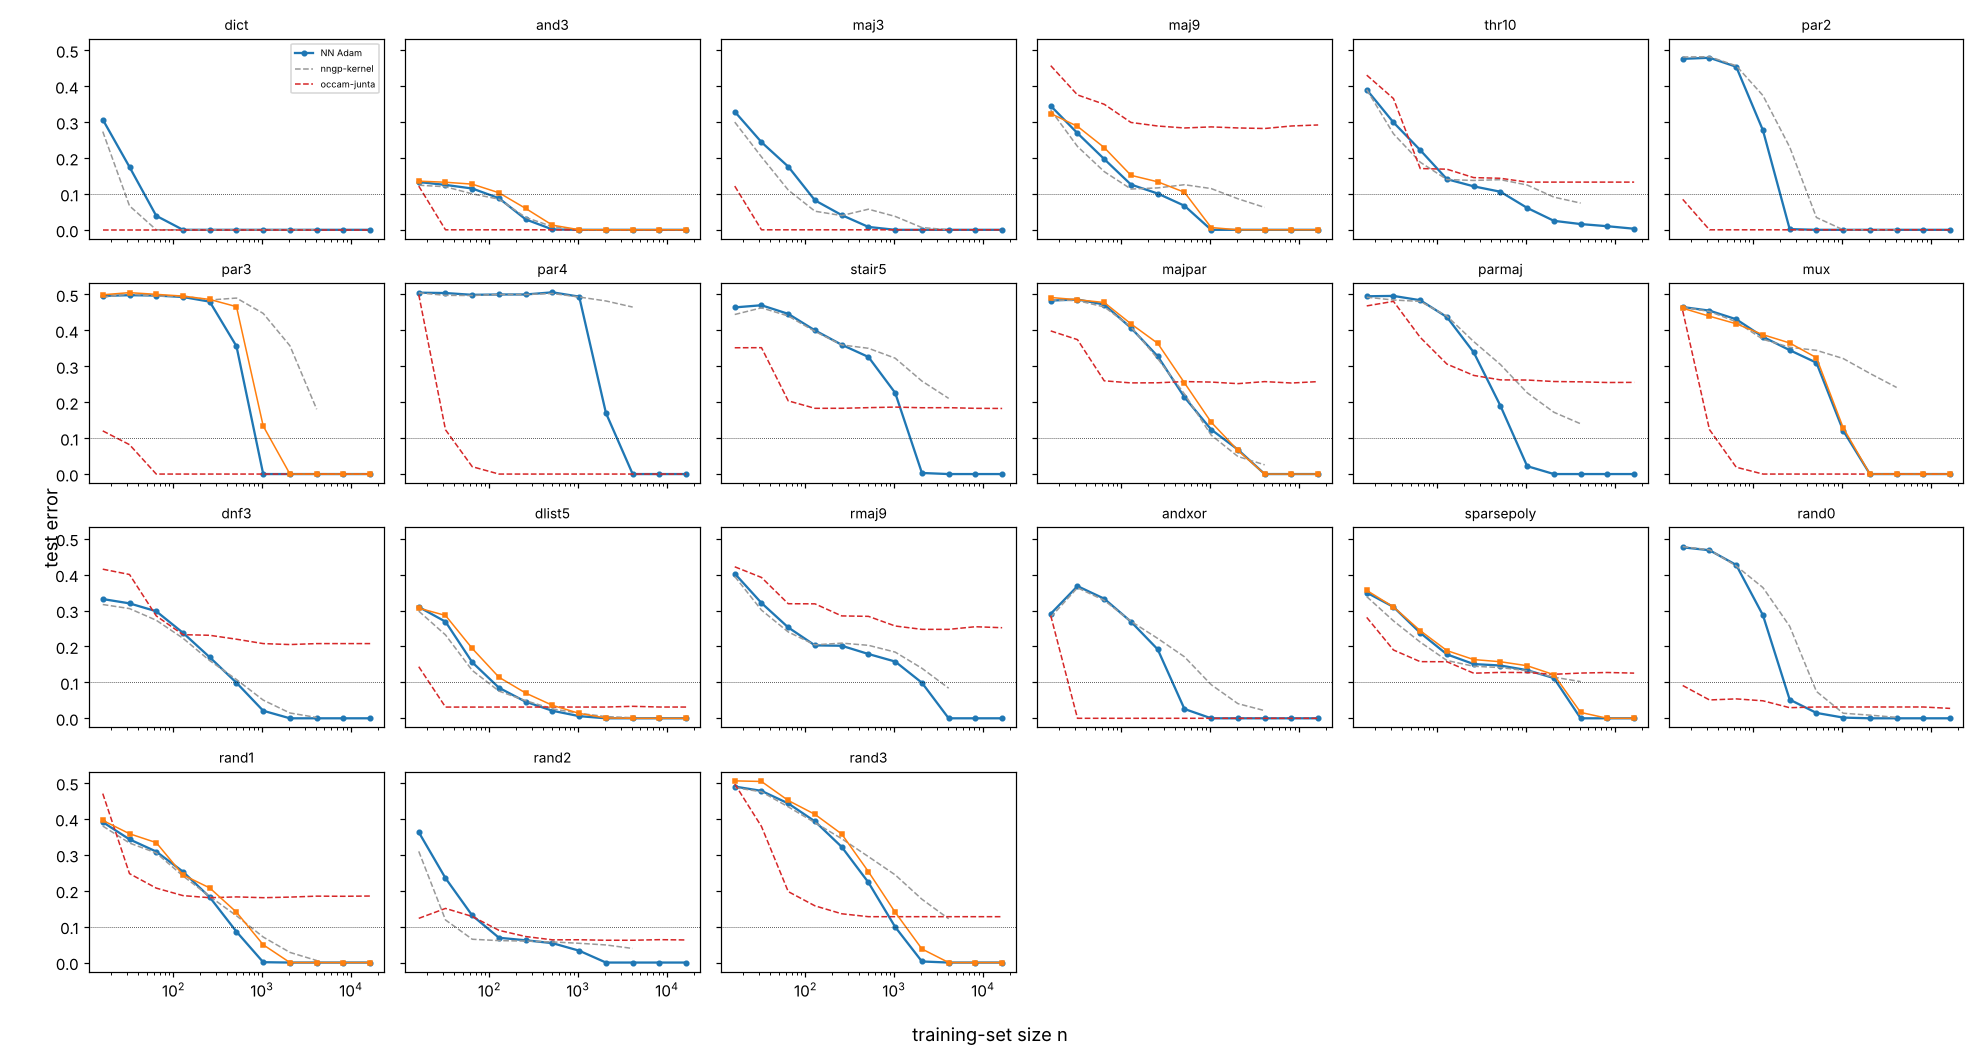
\includegraphics[width=\linewidth]{figures/nn_learning_curves.png}
\caption{Test error at the end of training against training-set size, $d=30$. Blue: Adam-trained networks (3 seeds). Orange: $\mu$P-SGD-trained networks, on the held-out targets (2 seeds). Grey dashed: NNGP kernel ridge regression. Red dashed: Occam over juntas of up to 4 variables.}
\label{fig:curves}
\end{figure}

Several further observations \status{Numerical}:
\begin{itemize}
\item \textbf{Reusing the training set saves data.} With fresh samples at every step, the networks need 12--64$\times$ their fixed-set $\nstar$: about 12800 samples for $\chi_2$, and about 32000 for $\chi_3$, the staircase, the multiplexer and MAJ of parities.
\item \textbf{Generalization is delayed near $\nstar$.} At $n=256$, $\chi_2$ fits its training set by step 200 but generalizes only at steps 7000--10000. The multiplexer, the DNF, recursive majority and AND$(x_1x_2,x_3x_4)$ show 4--40$\times$ delays at their critical $n$.
\item \textbf{Features are learned in staircase order.} On the staircase target, the network's Fourier coefficient reaches half its target value at step 100 for $x_1$, step 500 for $x_1x_2$ and $x_1x_2x_3$, and step 1000 for $x_1x_2x_3x_4$.
\item \textbf{Representation size peaks just below $\nstar$.} For the 3- and 4-bit parities, the staircase and the multiplexer, the participation-ratio rank of the second layer's kernel peaks just below $\nstar$ and collapses above it. Below $\nstar$ the networks fit the training set with many features; above it they use the target's few features.
\end{itemize}

\subsection{Dependence on the input dimension}\label{sec:dscale}

\Cref{tab:dscale} and \cref{fig:dscale} show $\nstar$ at $d=15,30,60$, and at $d=120$ for four targets \status{Numerical}. The growth with $d$ is polynomial, with an exponent that increases with the number of inputs that must be found at once:
\begin{itemize}
\item \textbf{Parities.} For 2- and 3-bit parities the exponents are $1.04$ and $1.91$ over $d=15$–$60$. On a refined grid of $n$ (quarter-octave steps), the local exponents from $d=30$ to $120$ are $1.09/1.03$ and $1.93/1.96$. Both match the CSQ rate $d^{\max(1,k-1)}$ \cite{abbe2023leap,benarous2021online}. The 4-bit parity grows like $d^{2.40}$, below $d^{3}$.
\item \textbf{Leap-1 compositions} (staircase, multiplexer) grow like $d^{1.5}$.
\item \textbf{MAJ$_9$.} Its whole learning curve is a function of $n/d$ at all four $d$, within 0.01–0.04 of a constant-free prediction from the sampling noise of the linear (Hebbian) direction (\cref{fig:dscale}b). Its apparent $\nstar$ exponent comes from where this flat curve crosses 0.1.
\end{itemize}
Occam-type laws grow like $\log d$, an effective exponent of about 0.2 over this range, and fail completely.

Training reuses a fixed sample for many epochs, so the networks are not CSQ learners in the strict sense. SQ algorithms, or gradient descent that reuses batches, can reach $d^{k/2}$ in Gaussian single-index models \cite{damian2024gaps,dandi2024reuse}. For $k\le3$ the networks here nevertheless follow the CSQ exponent; at $k=4$ they fall between the two rates.

\begin{table}[t]
\centering\small
\begin{tabular}{lccccc}
\toprule
target & $\nstar$ at $d=15$ / 30 / 60 / 120 & exponent ($15$–$60$) & CSQ $d^{k-1}$ & SQ/reuse $d^{k/2}$\\
\midrule
$\chi_2$ & 100 / 200 / 427 / 869 & 1.04 & 1 & 1\\
$\chi_3$ & 241 / 843 / 3410 / 10691$^\dagger$ & 1.91 & 2 & 1.5\\
$\chi_4$ & 508 / 2728 / 14255 / -- & 2.40 & 3 & 2\\
staircase (5 terms) & 433 / 1514 / 3487 / -- & 1.50 & -- & --\\
multiplexer & 364 / 1156 / 2848 / 5195$^\dagger$ & 1.48 & -- & --\\
MAJ$(x_1x_2,x_3x_4,x_5x_6)$ & 306 / 1380 / 3466 / -- & 1.75 & -- & --\\
MAJ$_9$ & 123 / 263 / 625 / 845 & 1.17 & -- & --\\
\bottomrule
\end{tabular}
\caption{Network sample complexity against input dimension (Adam, width 128; 3 seeds at $d=30$, 2 elsewhere). $^\dagger$On a refined (quarter-octave) $n$ grid; the factor-2 grid gives 14188 and 6524. For $\chi_4$ the 20000-step budget limits $\nstar$ at both ends of the range, so the sign of its effect on the exponent is unknown.}
\label{tab:dscale}
\end{table}

\begin{figure}[t]
\centering
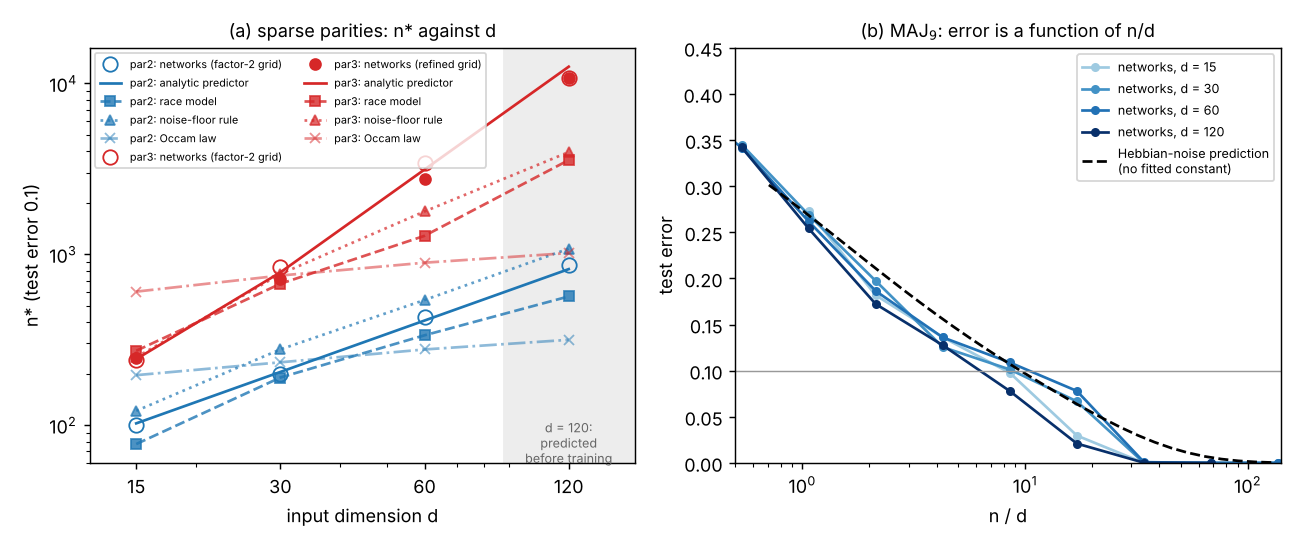
\includegraphics[width=\linewidth]{figures/understanding_dscale.png}
\caption{(a) $\nstar$ against $d$ for the 2- and 3-bit parities: networks, the analytic noise-law predictor (\cref{sec:noiselaw}), the race model, a noise-floor rule, and the Occam law. The predictions at $d=120$ (shaded) were saved before the $d=120$ networks were trained. (b) MAJ$_9$: network test error against $n/d$ at four input dimensions, and the constant-free prediction from the noise of the Hebbian direction.}
\label{fig:dscale}
\end{figure}

\subsection{Gradient descent against Occam, by leap}

Take the 26 targets, designed and random, with at most 4 relevant inputs. The ratio of the networks' $\nstar$ to the Occam-over-juntas learner's grows with the target's leap \status{Numerical}:

\begin{center}\small
\begin{tabular}{lcccc}
\toprule
leap & 1 & 2 & 3 & 4\\
targets & 14 & 8 & 2 & 2\\
median $\nstar_{\rm NN}/\nstar_{\rm Occam}$ at $d=30$ & 8.1 & 16.6 & 36 & 85\\
\bottomrule
\end{tabular}
\end{center}
Within leap 1 the spread is wide, from $1.7\times$ to $31\times$ (the multiplexer is $31\times$). The correlations along the target's greedy path matter as well as its leap. \Cref{sec:noiselaw} makes this quantitative.

\subsection{Robustness: optimizer and width}\label{sec:width}

\paragraph{SGD.} $\mu$P-SGD on the same training sets gives $\nstar$ similar to Adam's on the held-out targets: mean $|\log_2|$ ratio 0.43 \status{Numerical}. On the 3-parity, SGD needs 382, 1220 and 3562 samples at $d=15,30,60$, against Adam's 241, 843 and 3410. That is an exponent of 1.61 against 1.91. At $d=60$ both values are interpolated inside the same factor-2 step of the $n$ grid, so each exponent is uncertain by up to about $\pm0.25$, and the difference is not resolved.

\paragraph{Width.} At widths 32, 64, 128 and 256 (2 seeds; 3 at width 128) \status{Numerical}:
\begin{itemize}
\item \textbf{3-parity:} $\nstar$ does not change visibly (911, 827, 843, 873). At every width the test error is 0.28–0.47 at $n=512$ and exactly 0 at $n=1024$.
\item \textbf{4-parity:} $\nstar$ falls monotonically with width (3554, 3304, 2728, 1899), a factor of 1.9 from width 32 to 256, and has not levelled off.
\end{itemize}
This pattern does not fit a single width-dependent constant in the noise law of \cref{sec:noiselaw}, which would make the 4-parity's width effect the square of the 3-parity's. Nor does it fit a ``luckiest unit'' account. In that account the largest product of $k$ initial weights over the units would set the escape, and it predicts a width effect for the 3-parity too, since that maximum grows $1.9\times$ from width 32 to 256 at $k=3$. A guess \status{Heuristic}: the 3-parity is at its width limit by width 32, its escape carried by the bulk of the units as in mean-field theory, while the 4-parity still relies on lucky units.

\section{A discrete model of the feature channel}\label{sec:model}

\subsection{The race model}\label{sec:race}

The first model, the \emph{race model}, makes the saddle-to-saddle picture into an algorithm. Its parts:
\begin{itemize}
\item \textbf{State.} A shared two-level circuit of discrete ReLU gates $g=\mathrm{relu}(\sum_j w_ju_j-b)$. The weights are integers in $\{-3,\dots,3\}$, and the wires $u_j$ are input literals and earlier first-level gates. The gates feed a ridge least-squares readout, refitted after every new gate.
\item \textbf{Proto-units.} A persistent pool of dormant proto-units of orders 1–4 stands in for the not-yet-recruited hidden units.
\item \textbf{Alignment.} Each proto-unit's direction aligns to the residual by (tensor) power iteration on the training sample. It does so at the speed of the homogeneous law $\dot m=kU_km^{k-1}$, with $U_k$ the order-$k$ utility.
\item \textbf{Firing.} The rounded gate's utility then drives a clock, and the gate fires when the clock reaches $\theta=\log(1/\alpha)=1.5$. The earliest gate to fire is added to the circuit, the readout is refitted, and the race resumes.
\item \textbf{Stopping.} Growth stops at zero training error, or after 48 gates.
\end{itemize}
Three constants were calibrated on the 12 calibration targets only. The model sees nothing but the training sample.

\paragraph{Fit to the networks} \status{Numerical}. \Cref{tab:scoreboard} lists the scores.
\begin{itemize}
\item \textbf{Held-out targets.} The race model's $\nstar$ is within $1.26\times$ of the networks' on average, it ranks the targets identically, and its learning curves match in shape. It reproduces intermediate plateaus. For example, on sign$(2x_1+x_2x_3+x_4x_5x_6)$ test error stays near $1/8$ from $n\approx256$ to $n\approx2000$, which is the error of the partial predictor sign$(2x_1+x_2x_3)$.
\item \textbf{20 random formulas generated after calibration.} It is within $1.15\times$ on average (Spearman 0.99), better than on the held-out set.
\item \textbf{Other input dimensions.} At $d=15$ and $d=60$, without recalibration, it is within about $1.35\times$.
\item \textbf{The original ``mutate and keep improvements'' model.} A strong-selection/weak-mutation evolution of a single fan-in-2 circuit does much worse: mean $|\log_2|$ ratio 1.36.
\end{itemize}

\begin{table}[t]
\centering\footnotesize\setlength{\tabcolsep}{4pt}
\begin{tabular}{lcccccc}
\toprule
& \multicolumn{4}{c}{mean $|\log_2(\nstar_{\rm model}/\nstar_{\rm NN})|$} & & \\
\cmidrule(lr){2-5}
model & held-out (9) & random (20) & $d=15$ & $d=60$ & per-example & time Sp.\\
\midrule
race model & 0.33 & \textbf{0.20} & 0.45 & 0.43 & 0.50 & 0.83\\
race + kernel background (\cref{sec:hybrid}) & 0.35 & -- & 0.39 & 0.66 & 0.65 & 0.81\\
minimal model (2 constants) & 0.59 & 0.47 & 0.30 & 0.52 & 0.50 & 0.69\\
analytic predictor (no simulation) & 0.38 & 0.42 & 0.30 & 0.52 & -- & --\\
sswm (mutate and select) & 1.36 & 1.12 & -- & -- & 0.26 & 0.72\\
NNGP kernel & 2.58 & 1.78 & 1.43 & 2.68 & 0.69 & 0.22\\
Occam over juntas & 4.61 & 3.76 & -- & -- & 0.20 & $-0.07$\\
\midrule
\emph{SGD-trained vs Adam-trained networks} & \emph{0.43} & -- & -- & -- & \emph{0.71} & \emph{0.83}\\
\emph{Adam networks from a new initialization} & -- & -- & -- & -- & \emph{0.62} & --\\
\bottomrule
\end{tabular}
\caption{Models scored against the Adam-trained networks. Per-example agreement and the time Spearman are on the held-out targets. The race model's held-out score varies between 0.23 and 0.33 across its internal random streams; its value averaged over streams is 0.28. The hybrid's held-out $\nstar$ error is the average over its three streams; its other entries are for one stream (its agreement averaged over streams is 0.66). Its $d=60$ score uses a random-feature background above $n=2048$; with the exact kernel there it is 0.47. ``--'': not evaluated, or not defined for that model. The $d=15$ agreement of the minimal model and the predictor depends on a cap that was probably added after the $d=15$ network results had been seen, so it is not a clean out-of-sample test. The last two rows compare networks with networks.}
\label{tab:scoreboard}
\end{table}

\subsection{What makes it work: ablations}\label{sec:ablations}

\Cref{tab:ablations} summarizes 30 ablations, each run on the full grid with the calibrated constants and no recalibration \status{Numerical}. Every ``no change'' is judged against the model's own variation across its internal random streams, which spans 0.23–0.33 held-out over six streams.
\begin{itemize}
\item \textbf{The race dynamics do not set $\nstar$ on the held-out targets.} Removing the alignment cost, resetting the clocks after every firing, or replacing the race by plain greedy selection changes held-out $\nstar$ error by at most about 0.1 beyond that spread. So does varying $\theta$ from 0.5 to 6, the power-iteration steps from 1 to 32, or the pool size from 1 to 32. One exception: removing the alignment cost only for orders $\ge3$ gives 0.50. On the calibration targets, greedy selection (0.40), pool size 1 and one power-iteration step (0.49 each) sit 0.1–0.2 above the band of 0.23–0.30 there, mostly through the 4-parity. So how well the search reaches high-order directions does matter on that side. Compared model against model on the held-out targets, the alignment, clock, greedy and $\theta$ variants differ from the six control streams by 0.13–0.21 in $|\log_2\nstar|$, no more than the control streams differ from each other (0.11–0.23). Over all 21 targets, greedy (0.26), pool size 1 (0.32) and one power-iteration step (0.37) move more than a reseed does (0.10–0.21).
\item \textbf{The noise of the direction search does.} Computing the search directions on a large fresh sample removes their finite-sample noise. $\nstar$ then collapses to 16–87 on every target, as far from the networks as the Occam learner (4.63, against its 4.61). Running the whole search (directions, thresholds and utilities) on an independent sample of the \emph{same} size $n$ restores the match (0.31; directions alone: 0.41). So what matters is the noise \emph{level} at sample size $n$, not overfitting to the particular training labels.
\item \textbf{The particular sample's noise sets which examples are wrong.} With the independent search sample, per-example agreement falls from 0.50 to 0.26, although $\nstar$ is matched. Roughly half of the race model's excess agreement with the networks comes from both being misled by the same spurious correlations of the shared sample \status{Heuristic}.
\item \textbf{The gate library matters.} Without order-3 and order-4 candidates, the 3- and 4-bit parities, the sparse polynomial and recursive majority are never learned (1.43). Threshold gates in place of ReLU gates score 0.60, and weights in $\{-1,0,1\}$ score 0.81. Depth-2 gates help only staircase-like targets, by about 0.4 in $\log_2$.
\item \textbf{Time.} The ordering of targets by time to generalize survives every ablation, including the noise-free search, so the true features' utilities set it, not the race clocks. Within a target, the time Spearman is about 0.
\end{itemize}

\begin{table}[t]
\centering\footnotesize\setlength{\tabcolsep}{4pt}
\begin{tabular}{lcc}
\toprule
variant & held-out $|\log_2|$ ratio & per-example\\
\midrule
race model (calibrated) & 0.33 & 0.50\\
greedy: add the highest-utility gate, no race & 0.27 & 0.53\\
one alignment law for all orders & 0.28 & 0.50\\
depth-1 gates only & 0.35 & 0.51\\
two other internal random streams & 0.32, 0.27 & 0.51, 0.51\\
\midrule
noise-free search (directions from a large fresh sample) & 4.63 & 0.04\\
independent search sample of the same size $n$ & 0.31 & 0.26\\
no order-3/4 candidates & 1.43 & 0.52\\
\bottomrule
\end{tabular}
\caption{Selected ablations of the race model, held-out targets.}
\label{tab:ablations}
\end{table}

\subsection{The noise law and a closed-form predictor}\label{sec:noiselaw}

The ablations suggest a smaller model \status{Heuristic}: greedy stagewise least squares over ReLU gates with $\pm1$ weights, in which a candidate is accepted when
\begin{equation}\label{eq:noiselaw}
n\rho^2 \;>\; c\,N(k),\qquad N(k)=d\,\max\!\bigl(1,\tfrac da\bigr)^{\max(k-2,0)}\ (k\ge1),\qquad N(0)=|\text{active pool}|.
\end{equation}
\begin{itemize}
\item $\rho$ is the gate's correlation with the current residual.
\item $k$ is the number of inputs the gate needs that the circuit does not yet use. Reusing grown features ($k=0$) costs only a search over the small active pool.
\item For $k\ge3$ the heuristic derivation comes from the alignment law. An order-$k$ unit escapes only if its signal $kU m(0)^{k-1}$ beats the frozen sampling noise $\sim n^{-1/2}$, with an effective initial overlap $m(0)^2=a/d$. $N(1)=d$ is the sampling noise of the Hebbian unit, and $N(2)=d$ a spectral (BBP-type) threshold. The overlap reading of $a$ is not quantitative.
\end{itemize}
This is the correlational-SQ / leap scaling $d^{\max(1,k-1)}$. Two constants, $c=2.25$ and $a=18$, were calibrated on the calibration targets for the predictor and reused for the minimal model, whose own grid does not resolve its optimum. The predictor's structural choices were made with held-out scores in view.

Evaluated along the target's \emph{population} greedy path, \eqref{eq:noiselaw} gives a closed form:
\[
\nstar\approx\max\Bigl(n_{\rm Hebb},\ c\max_{i\le i^*}\frac{N(k_i)}{\rho_i^2}\Bigr).
\]
Here $i^*$ is the shortest prefix of the path that reaches error 0.1, and $n_{\rm Hebb}$ is the sampling-noise floor of the linear part. Some closed forms:
\begin{itemize}
\item $\nstar(x_1)=\Phi^{-1}(0.9)^2d=1.64\,d$, with no fitted constant.
\item $\nstar(\mathrm{MAJ}_9)=9.52\,d$, with no fitted constant.
\item $\nstar(\chi_k)=c\,(2^k-1)\,d\max(1,d/a)^{k-2}$. The first gate, AND$_k$, has $\rho^2=1/(2^k-1)$ with $\chi_k$, and the remaining gates are cheap $k=0$ moves.
\end{itemize}
On the 20 random formulas the analytic predictor, which reads $\nstar$ off its predicted learning curve, is within $1.34\times$ on average (Spearman 0.92–0.96, depending on the saved run). The closed form reproduces that curve's $\nstar$ for 19 of the 21 designed targets; it was not checked on the random formulas. The simulated minimal model keeps the race model's success agreement and per-example agreement, but not its held-out $\nstar$ accuracy (0.59, against an average of 0.28 for the race across its streams).

\paragraph{A pre-registered test at $d=120$} \status{Numerical}. The predictor, its variants, and the race model (4 internal streams) were evaluated at $d=120$ with their $d=30$ constants. Their predictions were saved before the $d=120$ networks were launched, and the file timestamps confirm the order.

\begin{center}\small
\begin{tabular}{lcccc}
\toprule
target & networks & analytic predictor & race model & Occam law\\
\midrule
$\chi_2$ & 869 & \textbf{817} & 566 & 315\\
$\chi_3$ & 10691 (refined grid) & \textbf{12525} & 3557 & 1015\\
MAJ$_9$ & 845 & 1143 & 1307 & 1143\\
multiplexer & 5195 (refined grid) & 3405 & 4013 & 891\\
\bottomrule
\end{tabular}
\end{center}
The 3-parity is the decisive case.
\begin{itemize}
\item \textbf{Predictor.} The leap law predicted that $\nstar$ would roughly quadruple from $d=60$ to 120. It did: from 2740 to 10691 on the refined grid.
\item \textbf{Race model.} From $d=30$ to 120 it grows only like $d^{1.2}$ ($2.8\times$ from 60 to 120), and it is now $3\times$ too optimistic. A possible reading \status{Heuristic}: its order-$k$ search accepts a direction once it is \emph{detectable} in the empirical moments, while the networks behave as if the direction must be \emph{reached} from a random start. A direct test of reachability from random starts does not explain the 3-parity gap at $d=60$, however.
\item \textbf{Why the race model matched at $d=30$.} At $d=30$ the two thresholds nearly coincide \status{Heuristic}.
\item \textbf{Misses of the predictor.} It underpredicts compositions of low-leap moves: the multiplexer by $1.5\times$ at $d=120$, and by $1.4$–$2.1\times$ at $d=30$ and 60. It overpredicts the 4-parity at $d=60$ by $1.6\times$.
\end{itemize}

\subsection{Kernel background plus grown features}\label{sec:hybrid}

The race model matches \emph{whether} and \emph{when} the networks generalize, but agrees less with \emph{which} test points they get wrong (0.50) than the NNGP kernel does (0.69). A diagnosis on the partially learned cells (95; most numbers below are on the 44 held-out ones) \status{Numerical}:
\begin{itemize}
\item \textbf{The output has two parts.} Split each learner's output into the part that depends only on the target's relevant variables, the signal, and the rest, which comes from the particular training sample. About 45\% of a network's output variance is this sample noise: 59\% at $n\le64$, 23\% at $n=2048$.
\item \textbf{Every learner gets the signal; the kernel gets the noise.} All learners match the network's signal part (correlation 0.92–0.98). The noise part correlates 0.81 with the kernel's, 0.70 with that of a network retrained from a new initialization, and 0.48 with the race model's.
\item \textbf{Swapping only the noise patterns} moves the race model's agreement from 0.50 to 0.63, and the kernel's from 0.69 to 0.53.
\item \textbf{Over training time,} the networks first interpolate within 100–1000 steps, with kernel-like mistakes. Near $\nstar$ the generalizing features grow afterwards.
\item \textbf{The kernel behaves like the network averaged over initializations.} Two single networks trained on the same data from different initializations agree only at 0.62. The average of three such networks agrees with a fourth at 0.684, and this extrapolates to about 0.71–0.73. The kernel agrees 0.78 with a three-network average.
\end{itemize}

A hybrid model adds an NNGP-kernel background to the race's gates in one joint ridge readout \status{Numerical}:
\begin{itemize}
\item \textbf{The background} relaxes on the race clock like kernel gradient flow, with ridge $c_{\rm bg}n/t$.
\item \textbf{Growth} stops at a square-loss level, $\texttt{stop\_mse}$, after which the background interpolates the remaining residual.
\item \textbf{Calibration.} Two constants, $c_{\rm bg}$ and $\texttt{stop\_mse}$, were chosen on the calibration set, together with the schedule form, the stop rule and the end-of-training step. Held-out agreement was visible while these design choices were explored, so only the constants are strictly calibrated on the calibration set.
\end{itemize}
Its results, and what they suggest:
\begin{itemize}
\item \textbf{Agreement.} On the held-out targets it raises per-example agreement from 0.50 to 0.65 (bootstrap over targets: $+0.15$, interval $[0.13,0.17]$). The gain holds on every held-out target and every seed.
\item \textbf{Cost.} Its $\nstar$ error is 0.35 against the race model's 0.28, both averaged over random streams.
\item \textbf{Few grown gates.} It needs about 2 grown gates per partially learned cell, where the race model needs about 22. The race model's extra gates memorize the sample. The networks do that with their random-feature background instead \status{Heuristic}.
\item \textbf{A simpler competitor does as well on these numbers.} Adding the race's and the kernel's standardized scores, each fitted separately, gives held-out $\nstar$ error 0.29 and agreement 0.62. The hybrid's advantage is mechanistic, not numerical: it is one learner, and its background does the memorizing in place of the race's extra gates.
\item \textbf{A candidate bound.} This suggests an a-priori bound of the form ``Occam for a few grown gates, plus a kernel-norm term for the background''. We have not attempted it.
\item \textbf{Remaining discrepancy.} On easy targets the networks are 1.1–2.2$\times$ \emph{less} sample-efficient than their own NNGP kernel, for example 47 against 29 samples for $x_1$. The race model reproduces this through its noisy Hebbian first gate; the hybrid does not.
\end{itemize}

\section{Does compositional structure beyond leap matter?}\label{sec:composition}
(Results pending.)

\section{What the network computes while it learns}\label{sec:trajectories}

Sections \ref{sec:networks}--\ref{sec:composition} concern \emph{whether} and \emph{when} the networks generalize. Here we ask \emph{what function} the network computes at each moment of training, and whether a general model reproduces the whole sequence of functions. Details are in \repo{study/trajectories/TRAJECTORIES.md}.

\paragraph{Setup.}
\begin{itemize}
\item \textbf{Targets.} Five chosen to differ in structure:
  \begin{itemize}
  \item sparsepoly $=\mathrm{sign}(2x_1+x_2x_3+x_4x_5x_6)$;
  \item a 5-term staircase;
  \item the multiplexer $x_4\,?\,x_1x_2x_3:\mathrm{MAJ}_3$;
  \item MAJ$(x_1x_2,x_3x_4,x_5x_6)$;
  \item MAJ of three MAJ$_3$.
  \end{itemize}
  Six held-out targets were run only after the models below were frozen.
\item \textbf{Conditions.} One-pass training, and fixed $n\in\{16384,2048,512\}$, with 3 seeds each.
\item \textbf{What is recorded.} At 72 log-spaced steps we record the network output on every pattern of the relevant variables $x_R$, each with 32 random settings of the irrelevant ones. This gives $f_R=E[f\mid x_R]$ exactly on the relevant cube, its full Fourier spectrum, and each target character's learned fraction $\varphi_S(t)=c_S(t)/\hat y_S$.
\end{itemize}

\begin{figure}[t]
\centering
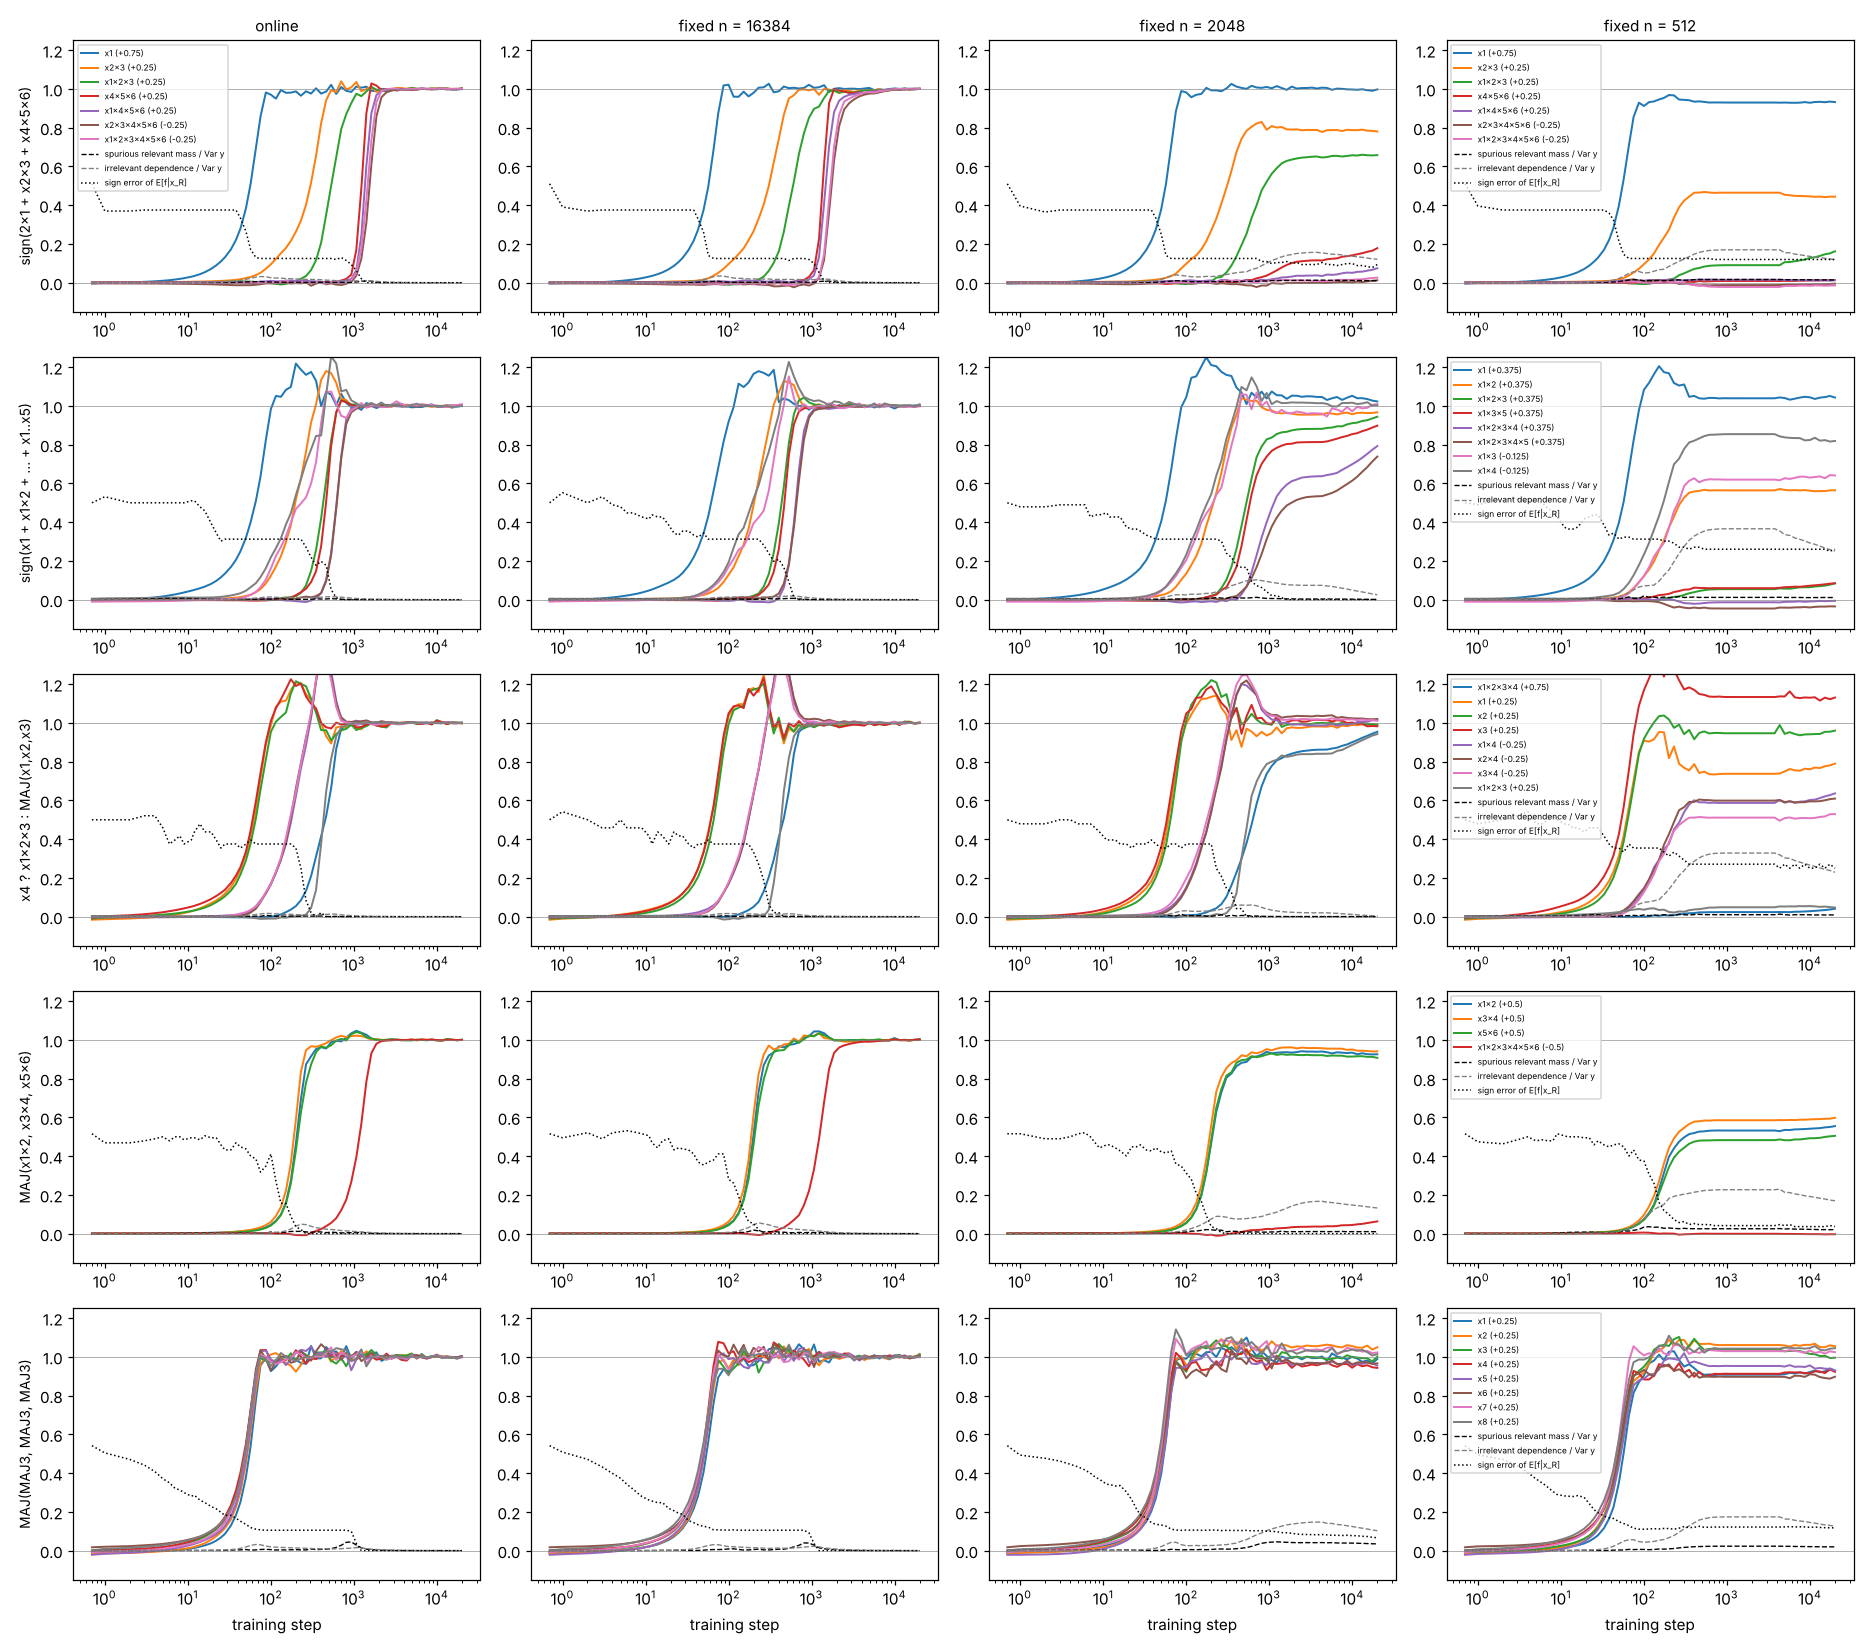
\includegraphics[width=\linewidth]{figures/trajectories.png}
\caption{Learned fraction of each Fourier character of the target (seed mean) against training step, for five targets (rows) and four conditions (columns). Dashed lines: spectral mass on characters the target does not have, and dependence on irrelevant inputs. Dotted line: sign error of $E[f\mid x_R]$.}
\label{fig:trajectories}
\end{figure}

\paragraph{The function on each plateau is a truncated Fourier expansion of the target} \status{Numerical}. On every plateau, $f_R$ is within 0.00–0.03 Var $y$ (at large $n$) of $P_{\mathcal S(t)}y=\sum_{S\in\mathcal S(t)}\hat y_S\chi_S$, the projection onto the characters learned so far.

The alternative ``the network fits everything about the inputs it has discovered'', $f_R\approx E[y\mid x_V]$, is 0.13–0.41 Var $y$ away on the same plateaus. For example, on MAJ$(x_1x_2,x_3x_4,x_5x_6)$ after the pairs, the distances are 0.003 against 0.225.

\paragraph{The sequence of functions} \status{Numerical} (\cref{fig:trajectories}).
\begin{itemize}
\item \textbf{Reproducibility.} The sequence is the same online and at $n=16384$, and seeds agree to about 15\% in onset step.
\item \textbf{The linear stage comes first,} at a nearly fixed 50–70 steps.
\item \textbf{Characters then arrive in bundles}, carried by one new feature direction:
  \begin{itemize}
  \item all $x_1x_j$ at once in the staircase;
  \item the three $x_ix_4$ in the multiplexer;
  \item about 500 characters of degree 2–8 in a 3-term DNF.
  \end{itemize}
\item \textbf{Order follows construction, not coefficient size.}
  \begin{itemize}
  \item The multiplexer's largest term, $x_1x_2x_3x_4$ (coefficient 0.75), comes last, after the features it is built from: steps 63, 172, then 437.
  \item In sparsepoly, $x_1$, $x_2x_3$, $x_1x_2x_3$ and $x_4x_5x_6$ (with its products) switch on at about 56, 297, 528 and 1389 steps.
  \end{itemize}
\item \textbf{Coefficients overshoot transiently,} by up to 1.36, as the readout refits on the features present.
\item \textbf{Finite $n$.} At finite $n$ the same sequence stops partway. Later stages saturate partially or never start, and memorization goes into the irrelevant inputs.
\end{itemize}

\paragraph{Three models} \status{Heuristic}. Each was calibrated on the five targets only, predicts $f_R(t)$ from the target alone, and was frozen (and committed) before any held-out network was run.
\begin{itemize}
\item \textbf{\texttt{fourier}, a by-hand rule.}
  \begin{itemize}
  \item \emph{Prediction.} $f_t=\sum_S\hat y_S\varphi_S(t)\chi_S$, with the fractions set by a race of \emph{moves}.
  \item \emph{Moves.} A move extends something already learned (nothing, a character, or a learned bundle) by $e$ new inputs at once. It learns every remaining character it reaches, as one bundle.
  \item \emph{Timing.} Duration $\propto\tau_0e^2\cdot2^{[\text{built on a feature}]}\cdot2^{[\text{odd degree}\ge3]}/\rho^{1/2}$, where $\rho$ is the bundle's share of the residual. A zero-bias ReLU gate has no first-layer gradient towards odd characters of degree at least 3.
  \item \emph{Finite $n$.} A memorization cut-off after a fixed number of epochs, and the spiked-estimation level $1-N/(n\rho^2)$.
  \end{itemize}
\item \textbf{\texttt{gates}.} A least-squares fit on greedily grown ReLU-gate bundles, with an alignment-law clock.
\item \textbf{\texttt{flow}.} The network's own Adam dynamics, reduced to the relevant inputs:
  \begin{itemize}
  \item the irrelevant inputs enter as Gaussian noise on each first-layer unit;
  \item the minibatch noise is kept in Adam's second moment;
  \item no constant is optimized against the networks.
  \end{itemize}
\end{itemize}

\begin{table}[t]
\centering\footnotesize\setlength{\tabcolsep}{4pt}
\begin{tabular}{lcccccc}
\toprule
& \multicolumn{3}{c}{calibration (5 targets)} & \multicolumn{3}{c}{held-out (6 targets)}\\
\cmidrule(lr){2-4}\cmidrule(lr){5-7}
traj against single seeds & online & $n=2048$ & $n=512$ & online & $n=2048$ & $n=512$\\
\midrule
\emph{network seed vs another seed} & \emph{0.0070} & \emph{0.0163} & \emph{0.0307} & \emph{0.0054} & \emph{0.0111} & \emph{0.0360}\\
\texttt{fourier} & 0.0087 & 0.0222 & 0.0188 & 0.0105 & 0.0177 & 0.0232\\
\texttt{gates} & 0.0096 & 0.0219 & 0.0196 & 0.0105 & 0.0205 & 0.0252\\
\texttt{flow} & 0.0042 & 0.0113 & 0.0208 & 0.0037 & 0.0097 & 0.0219\\
\bottomrule
\end{tabular}
\caption{Trajectory error, the mean over steps of $\lVert f_{\rm model}-f_{\rm net}\rVert^2/\mathrm{Var}\,y$, of each model against single network runs, next to one network run against another. A trivial step function (the target mean until step 1000, then the target) scores about 0.2.}
\label{tab:trajectories}
\end{table}

\paragraph{Results} \status{Numerical} (\cref{tab:trajectories}).
\begin{itemize}
\item \textbf{Out of sample.} All three models predict the held-out trajectories as well as the calibration ones.
\item \textbf{\texttt{flow}} predicts a network run better than an independent rerun of the network does, in every condition. Online, it puts held-out onsets within about 10\%.
\item \textbf{The two discrete rules} come within 1.3–2$\times$ of rerun-to-rerun variability at large $n$. \texttt{fourier}'s by-hand rule puts online onsets within about 25\%.
\item \textbf{Independent verification.} An agent per model regenerated every prediction bit for bit from the frozen commit, and found that no predictor reads any network data for the target it predicts. It also flagged two disclosures:
  \begin{itemize}
  \item the discrete rules have more tuned degrees of freedom than their five optimized constants: hand-tuned constants and structural switches chosen on calibration scores;
  \item the held-out targets, although new to this study, had been trained in the project's earlier fixed-$n$ study, whose data the models never read.
  \end{itemize}
\end{itemize}

\paragraph{Reading} \status{Heuristic}. The network computes a truncated Fourier expansion of the target and extends it in bundles. Each bundle is added by a move that builds on a feature it already has.
\begin{itemize}
\item \textbf{Cost.} A move is slower the more new inputs it must coordinate at once, and cheap when it composes existing features.
\item \textbf{Within a stage,} the readout refits on the features present.
\item \textbf{Finite $n$.} A race against memorization decides where the sequence stops.
\end{itemize}
This is the composition finding of \cref{sec:composition}, seen in time rather than in samples. The $e^2$ cost is a fixed-$d$ statement and does not include the $d^{k-1}$ dependence of \cref{sec:dscale}.

\section{Generalization bounds}\label{sec:bounds}

The question here is whether ``training has not taken long, so the circuit cannot have grown big, so a Chernoff bound over all small circuits applies'' can be made rigorous, and whether it gives useful numbers. \Cref{app:discrete,app:networks} state the results precisely. This section summarizes them.

\subsection{What is proved}

\paragraph{The Occam step needs no dynamics} \status{Proved}. Consider any learner whose output after $T$ gates is a circuit from a fixed library, followed by a threshold readout. In the realizable case its test error is at most about
\[
\bigl(T(\log|G|+k\log(d+T))+T^2\log2+\log\tfrac{(T+1)(T+2)}{\delta}\bigr)/n,
\]
simultaneously for all $T$ (\cref{app:discrete}). The dynamics are needed only to bound $T$.

\paragraph{Training time does not bound the raw gate count.} Many correlated gates can fire at once. On MAJ$_m$, $m^2$ gates fire at the same instant of the race. So training time cannot bound the raw gate count uniformly over gate libraries. For a fixed library only a weak time-only bound holds, with a factor of about $d$. What time does bound, in the race model, are three quantities \status{Proved}. Time is measured as $\tau(t)=\int_0^t\sqrt{2\hat L}$ in units of $\Theta=\log(1/\alpha)$, and the three quantities are:
\begin{itemize}
\item the circuit's depth;
\item its incoherence-weighted size, $T\le\kappa(\tau/\Theta)^2$, where $\kappa$ is the top eigenvalue of the fired gates' Gram matrix;
\item the readout's $\ell_1$ norm, at depth one.
\end{itemize}
Combined with the Occam step, they give statements of different strength. Besides the weak fixed-library bound, only the norm gives a test-error bound in training time alone, at depth one, and it is near-vacuous. The size bound is a decomposition: $\kappa$ is a property of the learned circuit, so the bound is never tighter than the Occam bound at the realized size. Depth alone bounds no test error. On targets with no depth-one correlation, such as parities, no gate fires before $t\approx\Theta\sqrt{n/(8\log M)}$. This is a precise version of ``it has not had time to memorize yet''. That noise gates in general start firing only around this time is \status{Heuristic}.

\paragraph{Diagonal linear networks} \status{Proved}. For a diagonal linear network over a Boolean feature dictionary, small-initialization gradient flow keeps the number of large coordinates at most $\kappa\,\tau^2/\Theta_\varepsilon^2$. This gives a generalization bound uniform in time, with only $\ln(\text{dictionary size})$ dependence.

\paragraph{Two-layer quadratic networks with fixed output signs} \status{Proved}. These are networks $f(x)=\sum_j[(u_j\cdot x)^2-\|u_j\|^2]-\sum_j[(v_j\cdot x)^2-\|v_j\|^2]=\langle UU^\top-VV^\top,xx^\top-I\rangle$, with output weights fixed at $\pm1$ and centred units, equivalently symmetric matrix sensing. Under gradient flow from small initialization, the number of grown hidden units is at most $\kappa(\tau/\Theta)^2$ at every training time.
\begin{itemize}
\item $\kappa$ depends only on the training inputs: not on the labels, the trajectory or the width.
\item The bound is weight-free rather than a-priori: $\tau$ is read off the training-loss curve. The same statement in raw training time alone is much weaker.
\end{itemize}
Together with a union bound over low-rank classes, this gives a test-error bound uniform in time. This makes the motivating sketch rigorous for this class of networks, in weight-free form. The bound loosens on plateaus with nonzero residual, where $\tau$ keeps growing.

\paragraph{Two-layer ReLU networks} (gradient flow from balanced small initialization). We prove three things \status{Proved}:
\begin{itemize}
\item an exact ``mass clock'' identity;
\item that no unit grows before about $\log(1/\alpha)/U^*$, with constant 1, which is sharp;
\item a width-free generalization bound valid through the first escape from the initial saddle. It is vacuous below about $n\approx10^5$ at $d=16$.
\end{itemize}
In addition:
\begin{itemize}
\item \textbf{Merging.} A conserved quantity, the off-diagonal part of the classical balancedness law \cite{arora2018optimization,du2018algorithmic}, makes same-sign neurons that share an activation pattern on the training set merge as their mass grows.
\item \textbf{Beyond the first escape.} Persistence of a small circuit holds under a condition that can be checked from the training residuals \status{Conditional}. The a-priori statement is open \status{Conjecture}.
\item \textbf{Reservoir depletion.} In small-$\alpha$ simulations ($\alpha\le10^{-3}$, width 64), the first escape recruited every neuron, except one in one run. In one run at $\alpha=10^{-6}$ the second feature was then not learned by $t=400$. The discrete models assume the reservoir of dormant units persists; whether it does in the $\mu$P networks was not measured.
\end{itemize}

\paragraph{One-pass training} \status{Proved}. With fresh minibatches, the prequential error certifies the average test error of a window of iterates, with no capacity argument \cite{cesabianchi2004online}. Taking the window in advance with $N$ fresh samples and $M$ prequential mistakes, the bound is $M/N+\sqrt{\ln(1/\delta)/(2N)}$.

\subsection{What can be certified for the trained networks}

\paragraph{Parameter-space bounds are vacuous or weak} \status{Numerical}. Norm-based and spectral bounds are vacuous at every $n\le16384$, the norm-based ones even at the initialization's norms. Mutual-information bounds are vacuous, and Hardt–Recht–Singer stability does not apply, because its assumptions fail. PAC-Bayes with a prior centred at initialization \cite{mcallester1999pacbayes,dziugaite2017computing} reaches 0.26–0.56 at $n=16384$ on the simplest targets only.

\paragraph{Distillation certificates are non-vacuous and never violated} \status{Proved method; Numerical results}. The method:
\begin{itemize}
\item Find a small circuit $g$ that agrees with the trained network on \emph{unlabelled} inputs. The candidates are a junta truth table, or the sign of a few Fourier characters with small integer weights.
\item Bound the network's test error by an Occam/Chernoff bound for $g$ on the training set, plus an upper confidence bound on the disagreement, estimated on unlabelled inputs not used to choose $g$.
\end{itemize}
No labelled hold-out data is used. Over all 21 targets, 5 training-set sizes and 3 seeds:
\begin{itemize}
\item 221 of 315 networks get a certificate below 0.5, and 163 one below 0.2.
\item No certificate falls below the network's actual test error.
\item At $n=16384$, every network is certified at 0.083 or less, except on three targets, where the certificate's circuit classes do not capture the network cheaply: MAJ of pair parities (0.54), sparse polynomial (0.29) and one random formula (0.42).
\item Over training time, the certificates track delayed generalization. On $\chi_3$ at $n=1024$, the network fits its training set by step 1000 with test error 0.165, and the certificate is 0.23. By step 20000 the test error is 0 and the certificate 0.073. While the network memorizes, the best certifying class temporarily grows, for example to signs of 8–10 characters, and then collapses to the 3-bit parity.
\end{itemize}

\paragraph{The race model's own circuits.} When the race model's circuit is small, its own-circuit Occam bound is tight: median 0.021 among generalizing fits with at most 6 gates. Half of its generalizing fits carry more than 6 gates, and those bounds are usually vacuous (median 0.67; 34\% are below 0.5). Yet most of these large circuits are \emph{functionally} small. A distillation certificate has median 0.125 on a sample of 30 and is below 0.2 in 24 of them. Size of representation and size of function come apart, for the model and for the networks alike.

\paragraph{Online.} On the one-pass runs, the prequential bound is within 0.01–0.18 of the test error at the end of each window throughout learning, and about 0.002 after learning. On MAJ$_9$ it is 0.53, 0.37, 0.20, 0.074, 0.032 and 0.013 over successive windows.

\subsection{What the bounds do not answer}
The bounds control the gap between training and test error. Once gradient descent generalizes, an Occam bound for the \emph{target's} circuit is already small in every case here: that circuit is tiny and $n\ge\nstar\gg k\log d$. The circuits actually found are often large in representation, and their own bounds weaker, as above. The binding question is therefore not the gap but \emph{how many samples until the feature is found}, i.e.\ the noise law of \cref{sec:noiselaw}:
\begin{itemize}
\item \textbf{Lower half.} For one-pass (CSQ-type) training, its lower half is the known CSQ rate \cite{abbe2023leap,abbe2021power}. For training that reuses a fixed sample, no matching lower bound is known, and the 4-parity data scale below $d^{k-1}$.
\item \textbf{Upper half.} For real networks, its upper half is open.
\end{itemize}

\section{Discussion}\label{sec:discussion}

\subsection{The picture}

Our current picture of rich-regime gradient descent on these targets \status{Heuristic}, summarizing the evidence of \cref{sec:networks,sec:model}:
\[
\text{trained network}\;\approx\;\underbrace{\text{random-feature kernel background}}_{\text{fits the sample noise; decides which examples are wrong}}\;+\;\underbrace{\text{a few grown features}}_{\text{decide whether and when it generalizes}}.
\]
Features are added greedily. A candidate is accepted once its correlation with the current residual beats the sampling noise of the \emph{continuous} search that would find it. That noise depends on how many inputs the feature needs at once that the circuit does not yet use, or, for a feature built from grown ones, how many existing features it must combine at once (\cref{sec:composition}); it grows polynomially in $d$. It is not the best-of-$M$ noise of a union bound over a finite library, so the cost is not a description length.

\subsection{Relation to NNBayes $\approx$ Occam}

\begin{itemize}
\item \textbf{The same answer to \emph{what} is learned.} Once gradient descent generalizes, the network is functionally close to a small circuit, as the distillation certificates show. So does the Occam picture predict \cite{nngen}.
\item \textbf{Different answers to \emph{how many samples}.}
  \begin{itemize}
  \item Occam pays the description length, about $k\log d$ for a $k$-parity. The $\gamma\ge1$ posterior of \cite{nngen} is proved to need only polynomially many samples; whether it pays only the description length is open.
  \item Gradient descent pays the noise cost of the most expensive move along its greedy path, about $d^{k-1}$ for a move that needs $k$ new inputs at once.
  \end{itemize}
\item \textbf{The gap grows with leap:} the median ratio is $8\times$, $17\times$, $36\times$ and $85\times$ at leaps 1–4, at $d=30$.
\end{itemize}
A conjecture suggested by the predictor, not shown here \status{Conjecture}: the two sample complexities are close for targets with a cheap greedy path, i.e.\ low-leap compositions with large residual correlations at every step. They differ by about $d^{k-1}/(k\log d)$ when a leap of size $k$ is unavoidable. For fixed $k$ that gap is itself polynomial; it becomes super-polynomial only if $k$ grows with $d$.

\subsection{What is in the literature, and what is new}

\paragraph{Known.} The qualitative picture is largely in the literature:
\begin{itemize}
\item the saddle-to-saddle / incremental-learning view of rich-regime gradient descent \cite{pesme2023saddle,jacot2021saddle,li2021greedy,kunin2025agf,bantzis2025saddle};
\item the leap / CSQ account of which sparse targets online SGD learns, and how fast \cite{abbe2022msp,abbe2023leap}, and its analogue for single-index models, the information exponent \cite{benarous2021online};
\item the equivalence of mutation-and-selection with CSQ learning \cite{feldman2008evolvability}.
\end{itemize}

\paragraph{New here, as far as we know.} The contributions are quantitative and empirical:
\begin{enumerate}
\item a calibrated discrete model and a two-constant closed form that predict per-target sample complexity of multi-epoch, fixed-sample training out of sample, including a pre-registered prediction at $d=120$;
\item ablations showing that the finite-sample noise level of the direction search, not the race dynamics, is the operative ingredient;
\item the kernel-background decomposition of the networks' mistakes;
\item the specific theorems of \cref{app:discrete,app:networks}: the weight-free rank bound for quadratic networks, and the early-phase results for ReLU networks;
\item the empirical finding that, for networks trained on a fixed sample, distillation certificates are the only tight bounds we found.
\end{enumerate}

\subsection{Leap counts supports, not structure}\label{sec:leapcritique}

Leap complexity is a function of the target's Fourier \emph{supports} only. Once the inputs of a monomial have been found, any further function of them is free in $d$. Leap therefore cannot see whether a high-order term can be built from intermediate features that are useful in their own right. Our move classification in \eqref{eq:noiselaw} inherits part of this blindness, since $k$ counts new inputs. But the correlation $\rho$ of the best available gate depends on which features already exist, so the noise law can in principle see such structure. An early version of this work proposed a ``circuit leap'' complexity. It orders a circuit's gates so that each insertion is a positive-utility move, and counts the largest number of gates that must be inserted at once. \Cref{sec:composition} tests the question directly.

\subsection{Limitations}
\begin{itemize}
\item \textbf{One setting.} All sample-complexity experiments use one architecture family (a $\mu$P two-hidden-layer ReLU MLP), mostly width 128 and Adam, square loss, uniform Boolean inputs, $d\le120$, and interactions of at most 4 bits. The theory checks use small two-layer ReLU, quadratic and diagonal linear networks.
\item \textbf{Width.} The 4-parity's width dependence is not explained by any model here (\cref{sec:width}).
\item \textbf{The noise law.} Its form for 3 or more simultaneous inputs is a fit, not a derivation. It misses the staircase, multiplexer and MAJ of parities by up to $2.1\times$, prices the reuse move of the composition test several times too cheaply (\cref{sec:composition}), and overpredicts the 4-parity at $d=60$.
\item \textbf{Training budget.} The networks' $\nstar$ is still falling at 20000 steps, by about 0.17 in $\log_2$ per doubling of training. Part of every match is a match at this training budget.
\item \textbf{Verification.} The theorems were checked by AI referees, not by humans (\cref{app:provenance}).
\end{itemize}

\subsection{Open problems}
\begin{enumerate}
\item \textbf{Prove the noise law} for a two-layer network trained on a fixed sample from small initialization: an order-$k$ feature escapes the plateau once $n\gtrsim d^{\max(1,k-1)}/\rho^2$, up to logarithms, with a matching lower bound for $k\le3$. For $k\ge4$ the networks scale below $d^{k-1}$, and the right exponent under sample reuse is open. Ingredients exist: information-exponent results for online SGD \cite{benarous2021online}, early alignment \cite{boursier2022early}, and the mass clock and merging law of \cref{app:networks}.
\item \textbf{Composition costs, and width dependence at order 4.}
\item \textbf{Reservoir depletion.} When does the first escape use up the dormant units at practical scales?
\item \textbf{A bound of the form ``Occam for a few grown features plus a kernel norm for the background''}, as suggested by the hybrid model.
\item \textbf{Bayes versus gradient descent.} Characterize the targets on which their sample complexities are close.
\end{enumerate}


\bibliographystyle{plainnat}
\bibliography{refs}

\appendix
\section{Bounds for the discrete circuit-growth model and for diagonal linear networks}
\label{app:discrete}

\begin{sloppypar}
This appendix states the results of two derivations: Sections A1--A4 of \repo{theory/A-discrete-model.md}, on the discrete circuit-growth model, and Sections C2--C3 of \repo{theory/C-bridge-and-certificates.md}, on diagonal linear networks and a conditional transfer to ReLU networks. Each was refereed twice, and the results are stated as revised after the second round. Numbering in parentheses is the derivation's. Proofs are sketched here; full proofs with explicit constants are in the derivations, and check scripts are in \repo{theory/checks}. ``Literature, from memory'' marks a published result whose statement the derivation could not check against the paper.
\end{sloppypar}

\subsection{Setting, counting and the Occam bound}\label{app:discrete:occam}

\paragraph{Notation.} $\mathcal X=\cube$, and $P$ is any distribution on $\mathcal X\times\{\pm1\}$, with input marginal $P_X$. The sample $S=((x_i,y_i))_{i\le n}$ is iid from $P$. We write $\langle u,v\rangle_n=\frac1n\sum_iu(x_i,y_i)v(x_i,y_i)$, $\|\cdot\|_n$ for its norm, and $\bar u=\langle u,1\rangle_n$ (in population statements, $\bar u=\E u$). The test error is $\mathrm{err}(h)=P(h(x)\ne y)$, and $\widehat{\mathrm{err}}$ is its value on $S$. Logarithms are natural. $\mathrm{kl}(q\|p)$ is the binary relative entropy, and $\mathrm{kl}^{-1}_+(q,\epsilon)=\sup\{p\ge q:\mathrm{kl}(q\|p)\le\epsilon\}\le q+\sqrt{2q\epsilon}+2\epsilon$. A test-error bound is \emph{useful} if it is at most $0.1$, and \emph{non-vacuous} if it is below $1/2$.

\paragraph{Circuits.} A \emph{library} $G$ is a finite set of gates $\phi:[-1,1]^j\to[-1,1]$ of arity $j\le k$. It is \emph{Boolean} if every gate maps $\{\pm1\}^j$ into $\{\pm1\}$. In a circuit with $T$ gates, gate $t$ applies some $\phi_t\in G$ to sources among the $d$ inputs and gates $1,\dots,t-1$, and computes $g_t$. A predictor $h=\psi(g_1,\dots,g_T)$ has a sign readout $\mathrm{sgn}(c_0+c\cdot z)$, an output-gate readout $\pm z_T$, or a real readout. $\mathcal H_T$ is the set of predictors with $T$ gates. A \emph{learner} is any rule, possibly randomized and data-dependent, that maps $S$ to circuits and readouts. The \emph{toy library} is $\{\mathrm{id},\mathrm{AND}(\pm a,\pm b),\mathrm{XOR}\}$ up to negation. It has $|G|=6$ and $k=2$, and at $d=30$ it has 2205 depth-one candidates.

\begin{lemma}[Counting (Lemmas 1.1, 1.2 in the derivation)]\label{lem:app-disc-count}
\status{Proved}\quad There are at most $e^{W_T}$ circuits with $T$ gates, where $W_T:=\sum_{t\le T}(\log|G|+k\log(d+t-1))$. On $N$ points of $\R^T$, at most $\Phi(N,T):=2\sum_{i\le T}\binom{N-1}{i}\le2N^T$ functions have the form $\mathrm{sgn}(c_0+c\cdot z)$. Hence $\log|\mathcal H_T|\le W_T+\rho_T$. Here $\rho_T=\log\Phi(2^{\min(T,d)},T)\approx T^2\log2$ (for $T\le d$) for a Boolean library with sign readout, $\rho_T=\log\Phi(2^d,T)$ for real-valued gates, and $\rho_T=\log2$ for an output-gate readout.
\end{lemma}

\begin{theorem}[Occam bound, uniform over circuit size (Theorem A1 in the derivation)]\label{thm:app-A1}
\status{Proved}\quad Fix $\delta\in(0,1)$ and let $L_T:=\log|\mathcal H_T|+\log\frac{(T+1)(T+2)}{\delta}$. With probability at least $1-\delta$ over $S$, every $T\ge0$ and every $h\in\mathcal H_T$ satisfy four bounds, where $p=\mathrm{err}(h)$ and $\hat p=\widehat{\mathrm{err}}(h)$:
\begin{enumerate}[label=(\arabic*),nosep]
\item if $\hat p\le p$, then $\mathrm{kl}(\hat p\|p)\le L_T/n$;
\item $p\le\hat p+\sqrt{2\hat pL_T/n}+2L_T/n$;
\item $p\le\hat p+\sqrt{L_T/2n}$;
\item if $\hat p=0$, then $p\le1-e^{-L_T/n}\le L_T/n$.
\end{enumerate}
A learner's output with $T(S)$ gates lies in $\mathcal H_{T(S)}$, however the gates were chosen. So the bounds hold for any learner, at every stage and every training time, with $T$ the number of distinct gate functions in use.
\end{theorem}
\begin{proof}[Proof sketch]
For a fixed $h$, the kl-Chernoff bound gives $P(\hat p\le p,\ \mathrm{kl}(\hat p\|p)>\epsilon)\le e^{-n\epsilon}$. Take a union bound over $\mathcal H_T$ with $\epsilon=L_T/n$, and then over $T$ with weights $\delta/((T+1)(T+2))$. Items (2)--(4) follow from $\mathrm{kl}(q\|p)\ge(p-q)^2/2p$, Pinsker's inequality, and $\mathrm{kl}(0\|p)=-\log(1-p)$. Nothing about the dynamics is used. This is the Occam argument~\cite{blumer1987occam}, made uniform over $T$.
\end{proof}

\paragraph{Values} \status{Numerical}. Take the toy library at $d=30$ and $\delta=0.05$.
\begin{itemize}[nosep]
\item $L_T=14.8$, $151$ and $427$ nats at $T=1$, $10$ and $20$.
\item The realizable bound (4) is useful for $T\le2,7,20,62$ and non-vacuous for $T\le11,27,102,403$, at $n=256,1024,4096,16384$.
\item The agnostic form (3) is weak: at $T=5$ and $n=4096$ its gap is $0.088$.
\item A symmetrization route in the style of Blumer, Ehrenfeucht, Haussler and Warmuth is larger at every $T\le1499$ for $n\in\{1024,4096,16384\}$.
\end{itemize}

\paragraph{A norm version} (Theorem A1$'$, \status{Proved given three textbook Rademacher lemmas}). This covers $f=c_0+\sum_jc_jg_j$ with $g_j$ in a finite class $\mathcal F$, $\sum_j|c_j|\le B$ and $|c_0|\le1+B$. Uniformly over $B=2^j$, with probability $1-\delta$, two gaps are bounded. The clipped square loss exceeds its empirical value by at most $4\mathfrak R_n(B)+2\sqrt{\log(2/\pi_j\delta)/2n}$. The 0-1 error exceeds the empirical ramp loss at a margin $\theta$ fixed in advance by at most $\frac2\theta\mathfrak R_n(B)+\sqrt{\log(2/\pi_j\delta)/2n}$. Here $\mathfrak R_n(B)=(1+B)/\sqrt n+B\sqrt{2\log(2|\mathcal F|)/n}$ and $\pi_j=1/((j+1)(j+2))$.

\subsection{The clock race and what training time controls}\label{app:discrete:time}

\begin{definition}[Clock race (Definition 2.1 in the derivation)]\label{def:app-race}
Fix $\Theta>0$. The state at time $t$ is a circuit of \emph{fired} gates, a readout $c(t)$, and the residual $r=y-f_t$, where $f_t=c_0+\sum c_mg_m$.
\begin{itemize}[nosep]
\item A \emph{candidate} $m$ is a gate on inputs or fired gates. Its \emph{availability time} $a_m$ is the last firing time among its gate sources, or $0$ if it has none.
\item Its \emph{clock} is $S_m(t)=\int_{a_m}^tU_m$, with utility $U_m=\langle r,g_m\rangle_n$. It fires when $|S_m|=\Theta$, with sign $\sigma_m=\mathrm{sgn}\,S_m$. Several candidates may fire at once, and clocks are never reset.
\item After each event the readout is refit, in one of two variants. (LS): least squares with an intercept over all fired gates. (SC), for a depth-one dictionary only: least squares with an intercept over $\mathrm{Sat}=\{m:|S_m|=\Theta\}$, subject to $\sigma_mc_m\ge0$.
\end{itemize}
\emph{Effective time} is $\tau(t)=\int_0^t\|r\|_n=\int_0^t\sqrt{2\hat L}$, and $R(t)=\int_0^tr$. The \emph{population race} uses $L^2(P)$ in place of the sample.
\end{definition}

\paragraph{Basic facts} (Lemma 2.2, \status{Proved}).
\begin{itemize}[nosep]
\item $|U_m|\le\|r\|_n\le1$, so $\tau\le t$.
\item In (LS), a fired gate keeps $U_m=0$.
\item In (SC), $|S_m|\le\Theta$.
\item With one threshold, rescaling $\Theta$ rescales time.
\end{itemize}
(SC) results hold up to any accumulation point of event times. Whether such points exist is open.

\paragraph{Scope.}
\begin{itemize}[nosep]
\item For moves needing $k=2$ fresh weight layers, $\Theta=c\log(1/\alpha)$, with a constant $c$ that depends on the parametrization ($c=\frac12$ for the diagonal network of \cref{app:discrete:diag}).
\item Fresh chains with $k\ge3$ cost about $\alpha^{-(k-2)}$, so the first move of a three-layer network started at scale $\alpha$ costs about $\alpha^{-1}$ \status{Heuristic}. The depth-one race therefore models diagonal or 2-homogeneous networks.
\item The diagonal network's small-$\alpha$ limit~\cite{pesme2023saddle} is recalled to match (SC) up to the intercept. AGF~\cite{kunin2025agf} also accumulates utility without resets. Both are Literature, from memory.
\item (LS) is not the depth-one limit.
\item Deeper moves are \status{Heuristic}.
\end{itemize}

\begin{proposition}[Depth (Proposition A2.1 in the derivation)]\label{prop:app-A21}
\status{Proved}\quad In either variant, a gate of depth $D$ fires only when $\tau(t)\ge D\Theta$. So the depth at time $t$ is at most $\lfloor\tau(t)/\Theta\rfloor\le\lfloor t/\Theta\rfloor$. The proof is by induction on $D$, since $\Theta=|S_m(t_m)|\le\tau(t_m)-\tau(a_m)$.
\end{proposition}

\begin{proposition}[No uniform gate-count bound (Proposition A2.2 in the derivation)]\label{prop:app-A22}
\status{Proved}\quad Consider the population race with uniform inputs and $y=\mathrm{MAJ}(x_1,\dots,x_m)$, for odd $m\le d$. Let $u_m=\binom{m-1}{(m-1)/2}2^{1-m}\approx\sqrt{2/\pi m}$.
\begin{enumerate}[label=(\arabic*),nosep]
\item For $G=\{\mathrm{id}\}$, $m$ gates fire together at $\Theta/u_m$ and nothing fires earlier, so $T\approx\frac2\pi(t/\Theta)^2$.
\item For the toy library, exactly $m^2$ functions, distinct up to sign, fire together at $\Theta/u_m$: the identities, $\mathrm{AND}(x_i,x_j)$ and $\mathrm{AND}(\neg x_i,\neg x_j)$. So $T\approx(\frac2\pi)^2(t/\Theta)^4$.
\item Duplicates with equal availability times fire together, so no function of $t/\Theta$ bounds the syntactic gate count uniformly over libraries.
\end{enumerate}
\end{proposition}
\begin{proof}[Proof sketch]
$\E[yx_i]=u_m$, the chance that the other votes tie, and $\E[yx_ix_j]=0$. Expanding the AND gates as $\mathrm{AND}(\epsilon_1a,\epsilon_2b)=(\epsilon_1a+\epsilon_2b+\epsilon_1\epsilon_2ab-1)/2$ shows that the listed gates have utility $\pm u_m$, and all others at most $u_m/2$ in absolute value.
\end{proof}
So no bound $T\le C(t/\Theta)^2$ with $C$ independent of $d$ holds for the toy library uniformly over the targets $\mathrm{MAJ}_m$, $m\le d$. At $n=4096$, maj3 fires 9 gates at $t/\Theta\in[1.98,2.12]$ \status{Numerical}.

\begin{theorem}[Gate count times incoherence (Theorem A2.3 in the derivation)]\label{thm:app-A23}
\status{Proved}\quad Let $K_B$ be the centred empirical Gram matrix of a set $B$ of gates, with entries $\langle g_m-\bar g_m,g_{m'}-\bar g_{m'}\rangle_n$, and $\kappa_B=\lambda_{\max}(K_B)$.
\begin{enumerate}[label=(\arabic*),nosep]
\item In (LS), at any depth, every set $B$ fired by time $t$ satisfies $|B|\le\kappa_B(\tau(t)/\Theta)^2$. If all $a_m=0$, $\tau$ may be replaced by $\|R(t)\|_n$.
\item In (SC), $|\mathrm{Sat}(t)|\le\kappa_{\mathrm{Sat}(t)}(\|R(t)\|_n/\Theta)^2$, and $\mathrm{supp}\,c\subseteq\mathrm{Sat}$.
\end{enumerate}
So the number $T(t)$ of distinct fired functions is at most $\kappa(t)(\tau/\Theta)^2$. Let $\mu_B$ be the largest absolute centred covariance within $B$, and $x=(\tau/\Theta)^2$. If $\mu_Bx<1$, then $|B|\le(1-\mu_B)x/(1-\mu_Bx)$, by Gershgorin's theorem.
\end{theorem}
\begin{proof}[Proof sketch]
Each $m\in B$ has $\sigma_mS_m(t)=\Theta$. The refit intercept gives $\bar r=0$, so $U_m=\langle r,\tilde g_m\rangle_n$ with $\tilde g_m=g_m-\bar g_m$. With $B(s)=\{m\in B:a_m\le s\}$, $|B|\Theta=\int_0^t\langle r,\sum_{B(s)}\sigma_m\tilde g_m\rangle_n\le\tau(t)\sqrt{\kappa_B|B|}$. The last step uses the fact that a principal submatrix has no larger top eigenvalue. When all $a_m=0$, apply Cauchy--Schwarz to $\langle R,\cdot\rangle_n$ instead.
\end{proof}
The population analogue is tight up to a factor $\pi/2$ (\cref{prop:app-A22}(1)). A library-wide coherence does not help, since the toy library has $\mu=\frac12$.

\begin{theorem}[$\ell_1$ norm of the readout (Theorem A2.4 in the derivation)]\label{thm:app-A24}
\status{Proved}\quad In (SC) on a depth-one dictionary, $\Theta\|c(t)\|_1=\langle R(t),f_t\rangle_n\le\|R(t)\|_n\sqrt{1-\bar y^2}\le\tau(t)$, and $|c_0|\le1+\|c\|_1$.
\end{theorem}
\begin{proof}[Proof sketch]
KKT gives $c_mS_m=|c_m|\Theta$, with $S_m=\langle R,g_m\rangle_n$. Since $\langle R,1\rangle_n=0$, $\Theta\|c\|_1=\langle R,f_t-\bar y\rangle_n$. Here $f_t-\bar y$ is the projection of $y-\bar y$ onto a cone, so its norm is at most $\sqrt{1-\bar y^2}$. This is LASSO duality, with $R$ as the residual and $\Theta$ as the penalty.
\end{proof}

\paragraph{Checks} \status{Numerical}. These are toy races at $d=30$ with $n=64$--$4096$.
\begin{itemize}[nosep]
\item \Cref{thm:app-A1,prop:app-A21,thm:app-A23} held at every event.
\item The ratio $\kappa\tau^2/(\Theta^2T)$ is $1.00$ on par2, where the bound is attained. It is at most 7 on maj3, and3 and dnf3, and up to 400 on par3, where one noise gate fires late.
\item \Cref{thm:app-A24} holds to machine precision in the toy (SC) runs, and to $3\cdot10^{-14}$ on 40 random correlated dictionaries with 130 exits from the saturated set.
\end{itemize}

\begin{corollary}[Test error along training (Corollary A2.5 in the derivation)]\label{cor:app-A25}
\status{Proved for (a), (a$'$); proved given the lemmas of A1$'$ for (b)}\quad Let $h_t=\mathrm{sgn}f_t$ and $D(t)=\lfloor\tau(t)/\Theta\rfloor$. Each of (a), (a$'$) and (b) holds with probability $1-\delta$, simultaneously for all $t$.
\begin{enumerate}[label=(\alph*),nosep]
\item For (LS), \cref{thm:app-A1} holds for $h_t$ with $T(t)\le\lfloor\kappa(t)\tau^2/\Theta^2\rfloor$. For example, at zero training error, $\mathrm{err}(h_t)\le L_{\lfloor\kappa\tau^2/\Theta^2\rfloor}/n$.
\item[(a$'$)] For (LS) or (SC), in a race that merges candidates equal up to sign on the sample: let $\mathcal F_{\le D}$ be the non-constant depth-$\le D$ functions that are distinct up to sign on the sample, and $\bar\kappa_D$ their top centred Gram eigenvalue. These depend only on the library and the unlabelled inputs. Then \cref{thm:app-A1} holds with $T(t)\le\min\{|\mathcal F_{\le D(t)}|,\lfloor\bar\kappa_{D(t)}\tau^2/\Theta^2\rfloor\}$, and at depth one $\tau$ may be replaced by $\|R\|_n$.
\item[(b)] For (SC) at depth one, Theorem A1$'$ holds with $B\le2\max(1,\tau/\Theta)$. Its gap is therefore of order $(1+\tau/\Theta)\sqrt{\log(|G|d^k)/n}$, whatever the gate count.
\end{enumerate}
\end{corollary}
For (a$'$), the fired representatives lie in $\mathcal F_{\le D(t)}$ (\cref{prop:app-A21}), and up to sign flips their Gram matrix is a principal submatrix of the library's.

\paragraph{How strong these are.}
\begin{itemize}[nosep]
\item \emph{(a) is a decomposition, not a time-only bound.} $\kappa(t)$ belongs to the learned circuit and can grow (3 for maj3 after its first event). It is never tighter than \cref{thm:app-A1} at the realized size.
\item \emph{(a$'$) is time-only but weak.} For the toy library, $\bar\kappa_1=d$ in the population, and $35$ and $32$ empirically at $n=4096$ and $16384$. At zero training error, (a$'$) gives $0.21$ and $0.053$ at $\|R\|_n=\Theta$, and $0.61$ and $0.195$ just below $2\Theta$. \Cref{thm:app-A1} at par2's realized size gives $0.004$ and $0.001$.
\item \emph{(a$'$) needs the merging.} A referee counterexample shows that it fails without it.
\item \emph{(b) is near-vacuous.} Its 0-1 bound at $n=4096$ is $0.40$--$0.97$.
\end{itemize}
So training time bounds the depth, the incoherence-weighted size and the depth-one readout norm. It bounds the raw gate count only through $\kappa(t)$ or $\bar\kappa\approx d$.

\subsection{Minibatches: reproducing the population run}\label{app:discrete:sgd}

\paragraph{The population greedy run (PG).} PG adds one gate per step. Given $C_t$, let $f_t$ be the $L^2(P)$ projection of $y$ onto $V_t=\mathrm{span}\{1,C_t\}$, and $r_t=y-f_t$. PG adds $m_t=\arg\max_m|U_t(m)|$, where $U_t(m)=\E[r_tg_m]$. The maximum is over $M_t\le|G|(d+t)^k$ candidates, identified up to sign. Three assumptions are made:
\begin{itemize}[nosep]
\item a gap $\gamma>0$: $|U_t(m_t)|\ge|U_t(m)|+\gamma$ for $m\ne\pm m_t$ and $t<T$;
\item $|r_t|\le R$;
\item $\lambda_*=\min_{t\le T}\lambda_{\min}(K_t)>0$, for the $L^2(P)$ Gram matrices $K_t$ of $(1,C_t)$.
\end{itemize}

\paragraph{The empirical run (EG).} At step $t$, EG uses a batch $B_t$ of size $b$: either $S$ itself (full batch) or a fresh batch. It refits on $B_t$, adds a maximizer of $|\langle\hat r_t,g_m\rangle_{B_t}|$, and outputs the sign of its final refit.

\begin{theorem}[Decision stability (Theorem A3.1 in the derivation)]\label{thm:app-A31}
\status{Proved}\quad Let $\epsilon=\gamma/(2+2\sqrt{2T/\lambda_*})$, and suppose that $b\ge\frac{2R^2}{\epsilon^2}\log\frac{4\sum_{t<T}(M_t+t+1)}{\delta}$ and $b\ge\frac{8(T+1)^2}{\lambda_*^2}\log\frac{4(T+1)^3}{\delta}$. Then, for both protocols, with probability $1-\delta$:
\begin{enumerate}[label=(\arabic*),nosep]
\item EG's circuit computes $C_T$;
\item if $y\in V_T$ almost surely, EG's predictor equals $y$ almost surely.
\end{enumerate}
With probability $1-2\delta$, \cref{thm:app-A1} holds for EG's predictor, on the sample of its final refit, with $L=\rho_T+\log(1/\delta)$ and no wiring term.
\end{theorem}
\begin{proof}[Proof sketch]
The functions $r_t$, $g_m$ and $K_t$ belong to the population run, so Hoeffding's inequality and a union bound give $\epsilon$-accurate empirical utilities, and $\lambda_{\min}(\hat K_t)\ge\lambda_*/2$. Inductively, if EG holds $C_t$, then $\hat r_t=(I-\hat\Pi_t)r_t$ with $\|\hat\Pi_tr_t\|^2<2(t+1)\epsilon^2/\lambda_*$. So every empirical utility is within $\gamma/2$ of $U_t$, and the gap fixes the argmax.
\end{proof}

\paragraph{Related results.}
\begin{itemize}[nosep]
\item \emph{Reuse} (Theorem A3.5, \status{Proved}). If batches are drawn with replacement from a fixed $S$ of size $n$, the same conclusions hold, with the Occam bound on $S$. The conditions use $(n^{-1/2}+b^{-1/2})^{-2}$ in place of $b$, and $\delta/2$ in place of $\delta$.
\item \emph{Thresholds} (\status{Numerical}). For par2, with $\mathrm{XOR}\in G$, $\gamma=\frac12$, $R=\lambda_*=1$ and $M_0=2205$, the theorem needs $b\ge2254$. With reuse at $n=16384$ it needs $b\ge6225$. So the experiments' $b=64$ is not covered. At $T=30$ and $\lambda_*=\frac12$, the Gram condition needs $4.5\cdot10^5$ samples.
\item \emph{Limits.} Stability gives exact recovery with no factor $1/\varepsilon$ for a target error $\varepsilon$, but it pays $1/\gamma^2$ and says nothing under ties or zero utilities.
\item \emph{The SGD race.} For the race, only clock concentration is proved (Lemma A3.2, \status{Proved}). Under fresh batches, with residuals bounded by $R$ and a fixed finite candidate set $\mathcal M$, with probability $1-\delta$ every clock stays within $R\sqrt{2\eta t_0\log(2|\mathcal M|/\delta)/b}$ of its drift clock up to time $t_0$; the observed errors are 75--88\% of this \status{Numerical}. That the race reproduces the population race is \status{Heuristic}.
\item \emph{Online-to-batch} (Proposition A3.3, \status{Proved}; cf.~\cite{cesabianchi2004online}). In one-pass training on fresh samples, pre-update minibatch losses estimate the trajectory's average test loss.
\end{itemize}

\subsection{Greedy growth versus minimum circuits}\label{app:discrete:greedy}

\begin{proposition}[Equal, overshoot, never (Propositions A4.1--A4.3 in the derivation)]\label{prop:app-A4}
\status{Proved; item 2 for the population race only}\quad Let $s^*$ be the size of the smallest consistent circuit.
\begin{enumerate}[label=(\arabic*),nosep]
\item If $y=\pm g^*$ for a depth-one candidate $g^*$, and $0<P(y=1)<1$, then $g^*$ and its duplicates fire first, at $\Theta/\mathrm{Var}(y)$. The race then stops with $T=1=s^*$. The same holds on a sample containing both labels, with $\mathrm{Var}_n$, and with duplicates meaning candidates equal to $\pm y$ on the sample.
\item Take uniform inputs, the toy library, and $y=\mathrm{maj}_3$. Then 9 gates fire at $2\Theta$, and the 0-1 error is already zero. Exactly 12 depth-two gates of utility $\frac14$ fire next, at $6\Theta$. So the race ends with 21 gates, while $s^*=3$ (\status{Numerical}, by exhaustive search). For $\mathrm{MAJ}_m$, $m^2$ gates fire where $m$ suffice.
\item Take uniform inputs and $y=\chi_A$ with $|A|=s>k$. Then nothing ever fires in the population race. On a sample, with probability $1-\delta$, nothing fires before $\Theta\sqrt{n/(8\log(2(M_1+1)/\delta))}$, where $M_1$ is the number of depth-one candidates (Proposition A2.6). If $\mathrm{XOR}\in G$, then with probability $1-\delta$ the minimum-consistent-circuit learner with an output-gate readout has error at most $L_{s-1}/n=O((s\log(d+s)+\log\frac1\delta)/n)$.
\end{enumerate}
\end{proposition}
\begin{proof}[Proof sketch]
(1) For $|g|\le1$, $|\E[(y-\bar y)g]|\le\E|y-\bar y|=\mathrm{Var}(y)$, with equality only for $g=\pm y$. (2) The 9 gates span the degree-$\le2$ functions, which leaves the residual $-\frac12x_1x_2x_3$, and a Fourier lemma bounds the depth-two utilities by $\frac14$. (3) Depth-one gates see fewer than $s$ variables, and the error bound is \cref{thm:app-A1}(4).
\end{proof}
So both learners get the same Occam bound as a function of $T$, and they differ in which $T$ they reach \status{Numerical}.
\begin{itemize}[nosep]
\item maj3 reaches zero training error with 6 gates at $n\ge256$.
\item dnf3 needs 18 gates where 6 suffice. Its bound at $n=4096$ is $0.084$, where 6 gates would give $0.019$.
\item par3 fires only noise gates, at $t/\Theta=2.65$--$20.0$ (the proved lower bound is $0.84$--$6.71$). Its bound of $0.52$--$0.95$ certifies nothing.
\end{itemize}

\subsection{Diagonal linear networks (Section C2 of the derivation)}\label{app:discrete:diag}

\paragraph{Setting.} The dictionary consists of $D$ characters $\chi_J(x)=\prod_{i\in J}x_i$; for example, taking all $|J|\le k$ gives $D=D_k=\sum_{i\le k}\binom di$. Let $X_{iJ}=\chi_J(x_i)$ and $K=X^\top X/n$. The model is $f_w=\sum_Jw_J\chi_J$, with $w=u\odot u-v\odot v$ and loss $L(w)=\frac1{2n}\|Xw-y\|^2$. It is trained by gradient flow from $u=v=\alpha\mathbf1$. Write $r=y-Xw$, $g=\nabla L=-X^\top r/n$, $G=\int_0^tg$, $\tau=\int_0^t\|r\|_n$ and $R=\int_0^tr$, and set $\Theta_\epsilon=\frac14\operatorname{arsinh}\frac\epsilon{2\alpha^2}\ge\frac14\log\frac\epsilon{\alpha^2}$.

\paragraph{Closed form and no early growth} (Lemma C2.1, Theorem C2.2, \status{Proved}).
\begin{itemize}[nosep]
\item $w(t)=-2\alpha^2\sinh(4G(t))$. So $-G_J$ is exactly the race clock, and $|w_J|\ge\epsilon$ exactly when it reaches $\Theta_\epsilon\approx\frac12\log\frac1\alpha$.
\item Since $|G_J|\le\tau$, nothing reaches $\epsilon$ while $\tau(t)<\Theta_\epsilon$.
\item Let $U_0=\max_J|\langle y,\chi_J\rangle_n|$ and $\epsilon_D=\sqrt{\lambda_{\max}(K)D}\,\epsilon$. If $U_0>\epsilon_D$, the first escape time lies in $[\Theta_\epsilon/(U_0+\epsilon_D),\Theta_\epsilon/(U_0-\epsilon_D)]$.
\end{itemize}

\begin{theorem}[How many coordinates can have grown (Theorem C2.3 in the derivation)]\label{thm:app-C23}
\status{Proved}\quad Let $B=\{J:|w_J(t)|\ge\epsilon\}$, $N_\epsilon=|B|$ and $\kappa_B=\lambda_{\max}(X_B^\top X_B/n)$.
\begin{enumerate}[label=(\arabic*),nosep]
\item $N_\epsilon\le(\int_0^t\|\nabla L\|_2)^2/\Theta_\epsilon^2$.
\item $N_\epsilon\le\kappa_B\tau^2/\Theta_\epsilon^2$. Let $\mu_n=\max_{J\ne J'}|\langle\chi_J,\chi_{J'}\rangle_n|$ and $x=(\tau/\Theta_\epsilon)^2$. Then $N_\epsilon\le(1-\mu_n)x/(1-\mu_nx)$ when $\mu_nx<1$. For uniform inputs and characters of degree at most $k$, with probability $1-\delta'$, $\mu_n\le\bar\mu:=\sqrt{2\log(2D_{\min(2k,d)}/\delta')/n}$.
\item $\sum_J|w_J||G_J|=\langle R,f_w\rangle_n$, so $\sum_{J\in B}|w_J|\le2\tau/\Theta_\epsilon$.
\end{enumerate}
\end{theorem}
\begin{proof}[Proof sketch]
Each $J\in B$ has $|G_J|\ge\Theta_\epsilon$, and (1) follows from Minkowski's inequality. For (2), with $\sigma_J=-\mathrm{sgn}\,G_J$, $N\Theta_\epsilon\le\int_0^t\langle r,\sum_B\sigma_J\chi_J\rangle_n\le\tau\sqrt{\kappa_BN}$, as in \cref{thm:app-A23}. The bound on $\mu_n$ is Hoeffding's inequality for the characters $\chi_{J\triangle J'}$.
\end{proof}
Item (2) is exact at the first crossing for a single-character target that is empirically orthogonal to the rest of the dictionary. At nonzero coherence it is strict; the derivation sketches, without a full proof, that it becomes tight as $\alpha\to0$.

\begin{theorem}[Generalization uniform in $t$ and $\epsilon$ (Theorem C2.4 in the derivation)]\label{thm:app-C24}
\status{Proved}\quad Let $\ell_N=\log\binom DN+\log\Phi(2^{\min(N,d+1)},N)$ and $\mu_\epsilon(t)=\sum_{J\notin B}|w_J(t)|$. With probability $1-\delta$, for all $t\ge0$ and $\epsilon>0$, with $N=N_\epsilon(t)$:
\[P(yf_{w(t)}\le0)\le\mathrm{kl}^{-1}_+\big(\widehat P_S[yf_{w(t)}\le2\mu_\epsilon(t)],\ (\ell_N+\log\tfrac{(N+1)(N+2)}\delta)/n\big).\]
\end{theorem}
\begin{proof}[Proof sketch]
Split $f_w=f_L+f_s$, with $f_L$ supported on $B$ and $\|f_s\|_\infty\le\mu$. The set $\{yf_L\le\mu\}$ is a threshold of $(y\chi_J(x))_{J\in B}$, which takes at most $2^{\min(N,d+1)}$ values. By Cover's count there are therefore at most $e^{\ell_N}$ such sets. Apply kl-Chernoff with a union bound over the sets and over $N$, and compare margins on test and training points.
\end{proof}

\begin{corollary}[Time-indexed form (Corollary C2.5 in the derivation)]\label{cor:app-C25}
\status{Proved}\quad Fix $\gamma\in(0,1]$. Let $\epsilon=\gamma/2D$, $\Theta_\gamma=\frac14\operatorname{arsinh}\frac{\gamma}{4D\alpha^2}$, $x=(\tau/\Theta_\gamma)^2$ and $\ell^*_N=\max_{N'\le N}\ell_{N'}$. On the event of \cref{thm:app-C24}, every $\bar N\in[N_\epsilon(t),D]$, possibly data-dependent, satisfies
\[\mathrm{err}(\mathrm{sgn}f_{w(t)})\le\mathrm{kl}^{-1}_+\big(\widehat P_S[yf_{w(t)}\le\gamma],\ (\ell^*_{\bar N}+\log\tfrac{(\bar N+1)(\bar N+2)}\delta)/n\big).\]
There are three admissible choices of $\bar N$, each capped at $D$:
\begin{enumerate}[label=(\arabic*),nosep]
\item $\lfloor\kappa_Bx\rfloor$, with $\kappa_B$ measured;
\item $\lfloor(1-\mu_n)x/(1-\mu_nx)\rfloor$, if $\mu_nx<1$;
\item for uniform inputs and all characters of degree $\le k$, the same with $\bar\mu$ in place of $\mu_n$, and optionally $t$ in place of $\tau$, if $\bar\mu x<1$, at total probability $1-\delta-\delta'$.
\end{enumerate}
\end{corollary}
Only choice (3) depends on $(n,D,\tau)$ alone, and it needs $n>2\log(2D_{\min(2k,d)}/\delta')(\tau/\Theta_\gamma)^4$. $D$ enters only through $\log D$.

\paragraph{Discrete GD and SGD} (Proposition C2.6, \status{Proved}). Suppose $2\eta\bar G<1$, where $\bar G=\max_j\|g_j\|_\infty$.
\begin{itemize}[nosep]
\item No coordinate grows before the minibatch effective time $\eta\sum_j\|r_j\|_{B_j}$ reaches $\Theta_\epsilon(1-4\eta^2\bar G^2)$.
\item Under SGD, the count is bounded only through the integrated gradient norms $\eta\sum_j\|g_j\|_2$, which is loose.
\item Under full-batch GD, the $\kappa_B\tau^2$ form holds, with $\Theta_\epsilon$ reduced by an explicit $O(\eta^2\bar G^2\tau)$.
\end{itemize}

\paragraph{Checks} \status{Numerical}. These are at $d=10$, $k=3$, $D=176$, with exact test errors. The generalization bounds are at $t=60$ and $\gamma=\frac12$.
\begin{itemize}[nosep]
\item \emph{Size bounds.} The worst ratio of $N$ to $\kappa_B\tau^2/\Theta^2$ is $0.33$--$0.94$, and $1.00$ for par2 at $\alpha=10^{-8}$. The discrete counts reach $0.62$--$0.80$ of their bound under GD, and only $0.07$--$0.12$ under SGD.
\item \emph{A posteriori.} At $\alpha=10^{-3}$, \cref{thm:app-C24} gives $0.107$ for par2 ($n=100$), $0.275$ and $0.077$ for maj3 ($n=100$ and $400$), and $0.166$ for and3 ($n=400$).
\item \emph{Time-indexed.} Choice (1) gives $0.218$, $0.810$, $0.316$ and $0.477$ on the same runs. Choices (2) and (3) are vacuous except for par2 at $\alpha=10^{-8}$, where they give $0.107$ and $0.163$. So the time-only form works here only for a single character at tiny $\alpha$.
\item \emph{Off-dictionary targets.} maj5 lies outside the dictionary and gets $0.951$, against a true error of $0.073$. par4 is uncorrelated with the dictionary and gets $0.988$.
\end{itemize}

\subsection{Conditional transfer to ReLU networks (Section C3 of the derivation)}\label{app:discrete:relu}

\paragraph{Known results and growth lemmas.} Rigorous results cover early alignment and the first escape in two-layer and homogeneous networks, for example~\cite{boursier2022early}. Exact saddle-to-saddle limits are known only for diagonal networks~\cite{pesme2023saddle,kunin2025agf} (Literature). The derivation proves one-sided growth bounds (Lemmas C3.1, C3.2, \status{Proved}). Let $\lambda_X$ be the top eigenvalue of the second moment of $(x,1)$.
\begin{itemize}[nosep]
\item \emph{Two layers.} In a two-layer ReLU network under gradient flow or descent, each unit's $\rho_j=a_j^2+\|w_j\|^2$ satisfies $\rho_j(t)\le\rho_j(0)e^{2\sqrt{\lambda_X}\tau(t)}$, with $\tau$ the discrete effective time $\eta\sum_k\|r_k\|_n$ for descent.
\item \emph{Deep networks.} In a bias-free deep ReLU network with $L\ge3$ under gradient flow, all layers grow equally~\cite{du2018algorithmic}. The quantity $Q=\max_l\|W_l(0)\|_F^2+\Delta$ satisfies $Q(t)^{1-L/2}\ge Q(0)^{1-L/2}-(L-2)\sqrt{\lambda_X}\tau$. So, with layers of Frobenius norm $\asymp\alpha$, escape takes effective time at least of order $\alpha^{-(L-2)}$.
\item \emph{Tightness} (\status{Numerical}). At $L=3$ this is loose by $14$--$21\times$, and at $L=4$ it is vacuous.
\item \emph{Scope.} The study's $\mu$P Adam networks are outside both lemmas.
\end{itemize}

\paragraph{The hypothesis.} Let $f_{\theta(t)}$ be the network at checkpoints $t\in\mathcal T$. Run the (LS) race on the same $S$ with a finite library. Let $h^M_s=\mathrm{sgn}f^M_s$ be its state at race time $s$, with $T^M(s)$ gates, and let $s(t)$ be a clock calibration. The \emph{saddle-to-saddle approximation hypothesis} (SSA) has two forms:
\begin{itemize}[nosep]
\item sign form: $P_X(\mathrm{sgn}f_{\theta(t)}\ne h^M_{s(t)})\le\eta(t)$;
\item $L^2$ form: $\|\mathrm{clip}f_{\theta(t)}-\mathrm{clip}f^M_{s(t)}\|_{L^2(P_X)}\le\eta(t)$.
\end{itemize}
For a Boolean library, let $L^{\rm sgn}_T=W_T+\log\Phi(2^{\min(T,d)},T)$ and $L^{\rm mar}_T=W_T+\log\Phi(2^{\min(T+1,d+1)},T+1)$. For real-valued gates the exponents are $d$ and $d+1$.

\begin{theorem}[The network inherits the race bound (Theorem C3.4 in the derivation)]\label{thm:app-C34}
\status{Conditional: proved under SSA}\quad There is an event of probability $1-\delta$ over $S$, not depending on the network, on which the following hold for every $t\in\mathcal T$. Here $s=s(t)$ and $T=T^M(s)\le\kappa^M(s)(\tau^M(s)/\Theta)^2$.
\begin{enumerate}[label=(\arabic*),nosep]
\item Under the sign form, $\mathrm{err}(\mathrm{sgn}f_{\theta(t)})\le\eta(t)+\mathrm{kl}^{-1}_+\big(\widehat{\mathrm{err}}_S(h^M_s),(L^{\rm sgn}_T+\log\frac{2(T+1)(T+2)}\delta)/n\big)$.
\item Under the $L^2$ form, for every $\gamma\in(0,1)$, $\mathrm{err}(\mathrm{sgn}f_{\theta(t)})\le\frac{\eta(t)^2}{\gamma^2}+\mathrm{kl}^{-1}_+\big(\widehat P_S[yf^M_s\le\gamma],(L^{\rm mar}_T+\log\frac{2(T+1)(T+2)}\delta)/n\big)$.
\end{enumerate}
\end{theorem}
\begin{proof}[Proof sketch]
Before training, fix two Occam events, each at level $\delta/2$: one for threshold-readout circuits, and one for margin sets of circuits. The sign form then adds the disagreement. In the $L^2$ form, $yf_\theta\le0$ forces either $yf^M\le\gamma$ or a clipped gap larger than $\gamma$, and Chebyshev's inequality bounds the latter.
\end{proof}

\paragraph{What this gives.}
\begin{itemize}[nosep]
\item \emph{A conversion only.} The theorem converts the hypothesis into a bound, and its size term is data-dependent through $\kappa^M$.
\item \emph{Testing SSA} (Corollary C3.5, \status{Proved}). Held-out unlabelled inputs make the sign form checkable. The distillation certificate (\cref{thm:C1}) then bounds the network with no hypothesis at all. So SSA is needed only for the predictive statement.
\item \emph{A first test} (\status{Numerical}). On the saved $\mu$P Adam networks, and3 and dnf3 match the race's constant state on their first plateau, which is trivial. In transitions, the best disagreement with any race state is $0.1$--$0.3$ (dnf3, mux, stair5), or no better than the disagreement with the target (maj3, majpar, parmaj). On par3 the race never starts, while the network learns.
\end{itemize}
So \cref{thm:app-C34} cannot yet be applied to the study's runs, and proving SSA beyond the first escape is open.

\section{Bounds for the trained networks}\label{app:networks}

This appendix collects the generalization bounds proved for actual networks, as opposed to the discrete race model. They come from three derivations:
\repo{theory/B-nn-time-bounds.md} (parameter-space bounds for the study's networks),
\repo{theory/C-bridge-and-certificates.md} (distillation certificates and the online protocol) and
\repo{theory/D-early-phase-theorem.md} (early-phase theorems for two-layer networks from small initialization).
Each derivation was refereed twice, and the second pass found only minor issues; the reports are \repo{theory/checks/referee_B_r2.json}, \repo{theory/checks/referee_C_r2.json} and \repo{theory/checks/referee_D_r2.json}.
Every result keeps its number from the derivation, given in parentheses. The status labels mean the following.
\status{Proved}: the derivation contains a complete proof with explicit constants, possibly invoking a named published result.
\status{Conditional}: proved under a stated hypothesis that is not itself proved.
\status{Conjecture}: not proved.
\status{Numerical}: a proved bound evaluated by a script whose output is in \repo{theory/checks/}.
The proof sketches give only the key idea.

\emph{Scope.} \Cref{app:networks:displacement,app:networks:norms,app:networks:pacbayes,app:networks:certificates,app:networks:online} concern the study's networks (three weight layers, $\mu$P initialization, SGD, GD or Adam). \Cref{app:networks:relu,app:networks:quad} concern two-layer networks trained from small initialization. None of D's theorems covers the study's $\mu$P Adam networks.

\subsection{Notation}\label{app:networks:notation}

\paragraph{Data, errors, kl.} Inputs are uniform on $\cube$ and labels are $y=f^\star(x)\in\{\pm1\}$. The sample $S=((x_i,y_i))_{i\le n}$ is iid. For predictors $h,g:\cube\to\{\pm1\}$ put $\mathrm{err}(h)=\Pr(h(x)\ne y)$ and $\mathrm{dis}(h,g)=\Pr_x(h(x)\ne g(x))$. Hats denote empirical versions on $S$ or on an unlabelled sample $U$, and $\widehat P_S[\cdot]$ is an empirical frequency on $S$. Write $\langle u,v\rangle_n=\frac1n\sum_iu(x_i)v(x_i)$ and $\|u\|_n^2=\langle u,u\rangle_n$. For real $f$, $\mathrm{err}(\mathrm{sgn}f)\le\Pr(yf(x)\le0)$, and the margin statements bound the right-hand side. $\mathrm{kl}(q\|p)$ is the binary relative entropy, and
\[
\mathrm{kl}^{-1}_+(q,c)=\sup\{p\in[q,1]:\mathrm{kl}(q\|p)\le c\}\ \le\ q+\sqrt{2qc}+2c .
\]
This inverse is nondecreasing in both arguments. Logarithms are natural.

\paragraph{The study's network.} Here $d=30$ and $f_\theta(x)=a\cdot\sigma(W_2\,\sigma(W_1x+b_1)+b_2)$, with $\sigma=\mathrm{relu}$ and hidden widths $N=128$.
\begin{itemize}
\item \emph{Parameters.} The groups $g=1,2,3$ are $(W_1,b_1)$, $(W_2,b_2)$ and $a$, with $p_g$ entries ($p=20608$ in total).
\item \emph{Initialization.} The $\mu$P initialization $\theta_0$ has $W_1\sim\mathcal N(0,1/d)$, $W_2\sim\mathcal N(0,1/N)$, $a\sim\mathcal N(0,1/N^2)$ and zero biases. It is drawn independently of $S$.
\item \emph{Losses.} $L_S(\theta)=\frac1{2n}\sum_i(f_\theta(x_i)-y_i)^2$, $L_0=L_S(\theta_0)\approx0.5$, and $R(\theta)=\Pr[yf_\theta(x)\le0]$.
\item \emph{Optimizers.} Every update has the form $\theta_{k+1}=\theta_k-\eta Mu_k$, where $M=\mathrm{diag}(m_g)$ holds the per-group $\mu$P multipliers. SGD ($\eta=0.2$, batch 64) and full-batch GD use gradients, with $m=(2,1,\frac12)$. Adam ($\eta=10^{-3}$) uses $u_k=\hat m_k/(\sqrt{\hat v_k}+\epsilon)$, with $m=(1,\frac12,\frac12)$.
\item \emph{Time and norms.} Training time is $t_K=\eta K$. The norms are $\|v\|_M^2=v^\top Mv$ and $\|v\|_{M^{-1}}^2=v^\top M^{-1}v$.
\end{itemize}

\subsection{Displacement from initialization as a function of time}\label{app:networks:displacement}

\begin{theorem}[Gradient flow; Theorem B1.1 in the derivation]\label{thm:B11}\status{Proved}
Let $\theta:[0,t]\to\R^p$ be absolutely continuous with $\theta'(s)=-Mv(s)$ for a.e.\ $s$, where $v(s)$ is a Clarke subgradient of $L_S$ at $\theta(s)$. Assume the chain rule $\frac{d}{ds}L_S(\theta(s))=\langle v(s),\theta'(s)\rangle$ a.e. (It is automatic for $C^1$ losses. For ReLU networks with square loss the derivation takes it from Davis--Drusvyatskiy--Kakade--Lee, FoCM 2020, quoted from memory.) Put $E_g(t)=\int_0^tm_g\|v_g\|^2ds$. Then:
\begin{enumerate}[label=(\arabic*)]
\item $\sum_gE_g(t)=L_S(\theta(0))-L_S(\theta(t))$;
\item $\|\theta(t)-\theta(0)\|_{M^{-1}}\le\Lambda(t):=\int_0^t\|\theta'\|_{M^{-1}}\le\sqrt{t\,(L_S(\theta(0))-L_S(\theta(t)))}\le\sqrt{tL_0}$;
\item $\|\theta_g(t)-\theta_g(0)\|^2\le m_g\,t\,E_g(t)$ for every group $g$.
\end{enumerate}
\end{theorem}
\noindent\emph{Sketch.} $\|\theta'\|_{M^{-1}}^2=v^\top Mv=-\frac{d}{ds}L_S$, which gives (1). Then apply the triangle inequality and Cauchy--Schwarz in $s$.

\begin{corollary}[Discrete time; Corollary B1.2]\label{cor:B12}\status{Proved}
(a) For any vectors $u_k$, $\|\theta_K-\theta_0\|_{M^{-1}}\le\Lambda_K:=\eta\sum_{k<K}\|u_k\|_M\le\sqrt{t_KE_K}$, where $E_K=\eta\sum_{k<K}\|u_k\|_M^2$. Per group, $\|\theta_{K,g}-\theta_{0,g}\|^2\le m_gt_KE_{K,g}$ with $E_{K,g}=\eta m_g\sum_k\|u_{k,g}\|^2$.
(b) For GD, suppose that for all $k<K$
\[
L_S(\theta_{k+1})\le L_S(\theta_k)-c\,\eta\,\|\nabla L_S(\theta_k)\|_M^2,\qquad c>0. \tag{D}
\]
Then $E_K\le(L_0-L_S(\theta_K))/c$, and so $\|\theta_K-\theta_0\|_{M^{-1}}\le\sqrt{t_K(L_0-L_S(\theta_K))/c}$.
\end{corollary}
\noindent Under $\beta$-smoothness in the $M$-geometry, (D) holds with $c=1-\beta\eta/2$. For ReLU networks no global $\beta$ exists, so (D) is an assumption about the trajectory. It can be checked a posteriori.

\begin{proposition}[SGD in expectation, smooth case; Proposition B1.3]\label{prop:B13}\status{Proved}
Assume that $L_S$ is $\beta$-smooth in the $M$-geometry on a convex set containing the iterates, and that $\eta\le1/\beta$. Assume that each minibatch gradient $\hat g_k$ averages $B$ per-example gradients at indices drawn uniformly with replacement, independently of the past, and that $\E[\|\hat g_k-\nabla L_S(\theta_k)\|_M^2\mid\mathcal F_k]\le\nu^2/B$. Then, with $t=\eta K$,
\[
\E\|\theta_K-\theta_0\|^2_{M^{-1}}\le4t\,(L_0-\E L_S(\theta_K))+2\eta t\nu^2(1+\beta t)/B .
\]
\end{proposition}
\noindent\emph{Sketch.} Split the displacement into drift and martingale noise. The cross terms of the noise vanish in expectation, and the drift is controlled by Cauchy--Schwarz and the descent lemma. The bound is weaker than \cref{thm:B11} by a factor of 4 and by a noise term that is quadratic in $t$. Its smoothness assumption fails for ReLU networks.

\begin{lemma}[Adam's exact worst-case step; Lemma B1.4]\label{lem:B14}\status{Proved}
Let $0\le\beta_1<1$ and $0<\beta_2<1$, with $r:=\beta_1^2/\beta_2<1$. For Adam's bias-corrected moments $\hat m_t,\hat v_t$ (coordinatewise, $m_0=v_0=0$), every gradient sequence and every $t\ge1$ satisfy
\[
\frac{|\hat m_t|}{\sqrt{\hat v_t}}\le C_t:=\frac{1-\beta_1}{1-\beta_1^t}\sqrt{\frac{1-\beta_2^t}{1-\beta_2}}\sqrt{\frac{1-r^t}{1-r}} ,
\]
with equality for $g_s\propto(\beta_2/\beta_1)^s$. Hence $\|\Delta\theta_g\|_\infty\le\eta m_gS_T$ after $T$ steps, where $S_T=\sum_{t\le T}C_t$.
\end{lemma}
\noindent\emph{Sketch.} Apply Cauchy--Schwarz to $m_t=(1-\beta_1)\sum_s\beta_1^{t-s}g_s$, splitting $\beta_1^{t-s}=(\beta_1/\sqrt{\beta_2})^{t-s}\sqrt{\beta_2}^{\,t-s}$. For $(\beta_1,\beta_2)=(0.9,0.999)$, $C_{100}=2.24$ and $C_\infty=7.27$, not the folklore value $1$. A geometric rise of the gradients, as at a saddle escape, exceeds $1$.

\paragraph{Numerical checks and vacuity.}\status{Numerical}
\begin{itemize}
\item \emph{A priori bounds are vacuous.} With no smoothness, the worst-case gradient-norm bound blows up after $5\times10^{-5}$ SGD steps (Remark B1.5). For Adam, \cref{lem:B14} allows $\|\Delta W_1\|_F\le8.9\times10^3$ after the study's 20000 steps, against a measured $4$--$11$.
\item \emph{Adam's ratio.} Real Adam runs reach a per-coordinate ratio $|\hat m|/\sqrt{\hat v}$ of $1.5$--$1.7$ during the first escape: $97\%$ and $94\%$ of $C_{50}$ at step 50 ($x_1$, MAJ$_3$).
\item \emph{Condition (D).} In a full-batch GD run at the study's rate (MAJ$_3$, $n=2048$, $\eta=0.2$), (D) holds only for the first 20 steps ($c_{20}=0.26$). At $\eta=0.02$ it holds throughout, with $c\ge0.993$.
\item \emph{The chain is loose.} For SGD at step 5000, $\|\Delta\|_{M^{-1}}=3.7$, $\Lambda=85$ and $\sqrt{tE}=159$.
\item \emph{Plateaus} (Heuristic). Time-only bounds degrade without limit as the initialization scale $\alpha\to0$, because plateau time grows while the learned function does not change.
\end{itemize}

\subsection{Why norm-based uniform convergence is vacuous here}\label{app:networks:norms}

Let $\varphi_\gamma(u)=\min(1,\max(0,1-u/\gamma))$ be the ramp loss, and $\hat R_\gamma(\theta)=\frac1n\sum_i\varphi_\gamma(y_if_\theta(x_i))$.

\begin{proposition}[Margin bound and its vacuity criterion; Theorem B2.1 and Lemma B2.1a]\label{prop:B21}\status{Proved}
Let $C(\theta)\ge0$ satisfy $\mathfrak R_n(\{f_\theta:C(\theta)\le\phi\})\le\kappa\phi/\sqrt n$ for all $\phi$. Fix $q>1$, $\phi_0>0$, $\gamma_{\max}$ and $\delta$. Put $\gamma_k=\gamma_{\max}q^{-k}$, $j(\theta)=\min\{j\ge0:\phi_0q^j\ge C(\theta)\}$ and $\delta_{jk}=\delta/((j+1)(j+2)(k+1)(k+2))$. With probability $\ge1-\delta$, for all $\theta$ and all $k\ge0$,
\[
R(\theta)\le\hat R_{\gamma_k}(\theta)+\frac{2\kappa\phi_0q^{j(\theta)}}{\gamma_k\sqrt n}+\sqrt{\frac{\ln(1/\delta_{j(\theta)k})}{2n}} .
\]
Let $c(\theta)=2\kappa\phi_0q^{j(\theta)}/\sqrt n$ and let $\bar m_+(\theta)=\frac1n\sum_i(y_if_\theta(x_i))_+$ be the mean positive train margin. If $c(\theta)\ge\max(1,\bar m_+(\theta))$, then the right-hand side is at least $1$ for every $k$, whatever $\gamma_{\max}$ is.
\end{proposition}
\noindent\emph{Sketch.} The first part is the margin bound of Koltchinskii--Panchenko (Mohri et al., Theorem 5.8), with a union bound over the two grids. For the second, $\varphi_\gamma(u)\ge1-u_+/\gamma$ gives $\hat R_\gamma\ge1-\bar m_+/\gamma$. Then split into the cases $\gamma_k\le1$ and $\gamma_k>1$.

The capacity constants are proved in the derivation for networks of any widths, with biases included.
\begin{itemize}
\item \emph{Path norm} (Proposition B2.2). For $\phi_1(\theta)=\sum_k|a_k|\bigl(\sum_j|W_{2,kj}|(\sum_i|W_{1,ji}|+|b_{1,j}|)+|b_{2,k}|\bigr)$, every $S\subset[-1,1]^d$ has $\hat{\mathfrak R}_S(\{\phi_1\le\phi\})\le\phi\sqrt{2\ln(8(d+1))/n}$, i.e.\ $\kappa_{\rm path}=3.32$.
\item \emph{Frobenius product} (Proposition B2.3). For $P_F(\theta)=\|a\|(\|[W_1\,b_1]\|_F\|W_2\|_F+\|b_2\|)$, every $S\subset\cube$ has $\hat{\mathfrak R}_S(\{P_F\le P\})\le\kappa_FP/\sqrt n$ with $\kappa_F=\sqrt{31}(1+\sqrt{4\ln2})=14.84$.
\end{itemize}
Both proofs rebalance the weights by positive homogeneity, peel the layers with exponential moments and the Ledoux--Talagrand comparison for convex increasing functions (Golowich--Rakhlin--Shamir's device), and finish with Hoeffding's or McDiarmid's inequality. A spectral bound (Bartlett--Foster--Telgarsky, with the initialization as reference matrices) is assembled in Theorem B2.4.

\paragraph{Numerical: vacuous for every network evaluated.}\status{Numerical} The bounds were evaluated on the 49 final Adam networks of the sweep, at $n\in\{256,2048,16384\}$. All of them have $\bar m_+=0.99$--$1.01$ and $c\ge\max(1,\bar m_+)$, so all three bounds are vacuous.
\begin{itemize}
\item \emph{Path norm.} The closest case is $c_{\rm path}=1.46$, for $x_1$ at $n=16384$.
\item \emph{Frobenius and spectral.} Over all 49 networks, $c_F=3.7$--$180$. The spectral complexity at unit margin is at least $679$.
\item \emph{The initialization alone is too large.} Already at the initialization's norms, $\phi_1(\theta_0)\approx(2/\pi)^{3/2}\sqrt{Nd}\approx31.5$ and $P_F(\theta_0)\approx\sqrt N\approx11.3$. This forces $c\ge1$ for $n\lesssim4.4\times10^4$ (path norm) and $n\lesssim1.1\times10^5$ (Frobenius).
\item \emph{A priori version.} Combined with \cref{thm:B11}, the Frobenius bound (Theorem B3.1) is vacuous even at $t=0$: $c_F=2.8$ at $n=16384$ and $22$ at $n=256$.
\end{itemize}
\emph{Heuristic reading:} the norms are dominated by the random features present at initialization. It is not a theorem, and training can lower the norms: the path norm of $x_1$ at $n=16384$ is $26$ after training and $32$ at initialization.

\subsection{PAC-Bayes centred at the initialization}\label{app:networks:pacbayes}

Let $\Sigma$ be a finite grid of per-group noise levels $\sigma=(\sigma_1,\sigma_2,\sigma_3)$, with $|\Sigma|=G$. Put $Q_{\theta,\sigma}=\mathcal N(\theta,\mathrm{diag}(\sigma_g^2I_{p_g}))$ and $P_\sigma=\mathcal N(\theta_0,\mathrm{diag}(\sigma_g^2I_{p_g}))$, and let $\mathrm{KL}=\sum_g\|\theta_g-\theta_{0,g}\|^2/2\sigma_g^2$ be their relative entropy.

\begin{theorem}[PAC-Bayes with the prior at initialization; Theorem B3.2]\label{thm:B32}\status{Proved}
Let $n\ge8$. With probability $\ge1-\delta_0$, for all $\theta$ (however obtained) and all $\sigma\in\Sigma$,
\[
R(Q_{\theta,\sigma})\le\mathrm{kl}^{-1}_+\Bigl(\hat R_S(Q_{\theta,\sigma}),\ \tfrac1n\bigl[\mathrm{KL}+\ln\tfrac{2G\sqrt n}{\delta_0}\bigr]\Bigr). \tag{PB}
\]
\emph{Derandomized form.} Suppose $\theta$ and $\sigma$ are fixed first, by any rule. Then draw, independently of that choice, $m$ iid pairs $(\theta'_j,B_j)$ with $\theta'_j\sim Q_{\theta,\sigma}$ and $B_j$ a batch drawn from $S$. Let $\hat e$ be the mean batch error, and $\hat\Delta$ the mean sign disagreement of $f_{\theta'_j}$ and $f_\theta$ on $m$ fresh batches of unlabelled uniform inputs. With probability $\ge1-\delta_0-\delta_1-\delta_2$,
\[
R(\theta)\le\mathrm{kl}^{-1}_+\Bigl(\mathrm{kl}^{-1}_+\bigl(\hat e,\tfrac{\ln(1/\delta_1)}m\bigr),\ \tfrac1n\bigl[\mathrm{KL}+\ln\tfrac{2G\sqrt n}{\delta_0}\bigr]\Bigr)+\mathrm{kl}^{-1}_+\bigl(\hat\Delta,\tfrac{\ln(1/\delta_2)}m\bigr).
\]
\end{theorem}
\noindent\emph{Sketch.} The prior depends only on $\theta_0$, which is independent of $S$. So the PAC-Bayes-kl bound (Maurer 2004, Theorem 5; in the line of \cite{mcallester1999pacbayes}) applies conditionally on $\theta_0$, with a union bound over $\Sigma$. The Monte Carlo terms use kl-Chernoff on the fresh draws. Derandomization uses $\mathbb 1[yf_\theta\le0]\le\mathbb 1[yf_{\theta'}\le0]+\mathbb 1[\mathrm{sgn}f_{\theta'}\ne\mathrm{sgn}f_\theta]$. The approach is that of \cite{dziugaite2017computing}, with the prior centred at the initialization.

\begin{theorem}[Time-based KL: ``short training implies generalization''; Theorem B3.3]\label{thm:B33}\status{Proved}
Under the hypotheses of \cref{thm:B32}, with $\lambda_\sigma=\max_gm_g/2\sigma_g^2$, the KL in (PB) at the trained parameters satisfies:
\begin{enumerate}[label=(\alph*)]
\item for gradient flow, or GD under (D) with constant $c$ ($c=1$ for the flow): $\mathrm{KL}\le t(L_0-L_S(\theta(t)))\lambda_\sigma/c\le tL_0\lambda_\sigma/c$, which is linear in time;
\item for any update: $\mathrm{KL}\le t_K\sum_gm_gE_{K,g}/2\sigma_g^2$, with the measured energies of \cref{cor:B12}(a);
\item for Adam: $\mathrm{KL}\le\sum_gp_g(\eta m_gS_K)^2/2\sigma_g^2$, which is quadratic in $K$, since $S_K\ge K$;
\item for SGD, under the hypotheses of \cref{prop:B13}, with $V(t)=4tL_0+2\eta t\nu^2(1+\beta t)/B$: with probability $\ge1-\delta_0-\delta'$ over $S$ and the minibatches, (PB) holds at $\theta_K$ with $\mathrm{KL}\le\lambda_\sigma V(t)/\delta'$; and the randomized predictor ``rerun SGD, then perturb'' satisfies the PAC-Bayes-kl inequality with $\mathrm{KL}\le\lambda_\sigma V(t)$.
\end{enumerate}
\end{theorem}
\noindent\emph{Sketch.} $\mathrm{KL}\le\lambda_\sigma\|\theta-\theta_0\|^2_{M^{-1}}$. Insert \cref{thm:B11}, \cref{cor:B12} or \cref{lem:B14}. For (d), insert \cref{prop:B13} together with Markov's inequality, or with convexity of KL for the mixture.

\paragraph{Numerical.}\status{Numerical}
\begin{itemize}
\item \emph{Final Adam networks} (20000 steps). For the deterministic network, the bound is $0.26$--$0.56$ at $n=16384$ for the five targets with at most three relevant variables ($x_1$, AND$_3$, MAJ$_3$, $x_1x_2$, $x_1x_2x_3$). It is $0.55$--$1.0$ at $n=2048$, and vacuous at $n=256$. For targets with 4--6 relevant variables it is uninformative even at $n=16384$ ($0.79$--$1.0$; KL $3500$--$6000$ nats). For $x_1$ at $n=16384$ the KL is $1804$ nats, against about 4 nats for describing $x_1$ in any circuit language.
\item \emph{Early checkpoints.} After 100--300 steps of SGD or Adam at $n=16384$ the bounds are $0.10$--$0.34$. With a union bound over the 10 checkpoints evaluated per target, the best are $0.11$ ($x_1$) and $0.23$ (MAJ$_3$).
\item \emph{Time-based forms.} These are informative ($<0.5$) only up to gradient-flow time $t\approx4$, or 50 Adam steps.
  \begin{itemize}
  \item (a), GD at $\eta=0.02$: $0.59$--$0.77$ over steps 200--1000.
  \item (b): $0.39$ for SGD on $x_1$ at step 20, then at least $0.9$ from step 100 on. (b) is a diagnostic, always weaker than (PB) with the measured displacement; its KL is $2$--$44$ times the flow value.
  \item (c), Adam: $0.44$--$0.56$ at step 50, and vacuous by step 200.
  \item (d) is not evaluated, because smoothness fails for ReLU.
  \end{itemize}
\end{itemize}

\subsection{Distillation certificates without labelled hold-out data}\label{app:networks:certificates}

\paragraph{Setting.} $\{\mathcal H_c\}_{c\in I}$ is a countable family of finite classes of predictors $\cube\to\{\pm1\}$, with weights $\pi(c)>0$, $\sum_c\pi(c)\le1$, all fixed before seeing data. Training randomness $\xi$ is independent of $S$. The predictors to be certified, $h_1,\dots,h_J$ (for example checkpoints), are arbitrary functions of $(S,\xi)$. $U=(u_1,\dots,u_m)$ is iid from the input distribution and independent of $(S,\xi)$.

\begin{theorem}[Distillation certificate; Theorem C1]\label{thm:C1}\status{Proved}
With probability $\ge1-\delta_1-\delta_2$ over $(S,\xi,U)$, simultaneously for every $j\le J$, every $c\in I$ and every $g\in\mathcal H_c$ (in particular for a $g$ selected using $S$, $\xi$, $h_j$ and $U$),
\[
\mathrm{err}(h_j)\le\mathrm{kl}^{-1}_+\bigl(\widehat{\mathrm{err}}_S(g),\varepsilon^S_c\bigr)+\mathrm{kl}^{-1}_+\bigl(\widehat{\mathrm{dis}}_U(h_j,g),\varepsilon^U_c\bigr),
\qquad
\varepsilon^S_c=\tfrac{\ln|\mathcal H_c|+\ln\frac1{\pi(c)}+\ln\frac1{\delta_1}}n,\quad
\varepsilon^U_c=\tfrac{\ln|\mathcal H_c|+\ln\frac1{\pi(c)}+\ln\frac J{\delta_2}}m .
\]
(b) If a list of $K$ candidates $(c_k,g_k)$ is chosen from $(S,\xi,U_A)$, and $U_B$ ($m_B$ points) is independent of $(S,\xi,U_A)$, then $\varepsilon^U$ may be replaced by $\ln(JK/\delta_2)/m_B$.
(c) If $\mathrm{dis}(h_j,g)$ is computed exactly, the second term is $\mathrm{dis}(h_j,g)$, at probability $1-\delta_1$.
\end{theorem}
\noindent\emph{Sketch.} The Occam event, a kl-Chernoff and union bound over all of $\bigcup_c\mathcal H_c$ \cite{blumer1987occam}, involves neither $h$ nor the selection rule. So $g$ may be fitted to $h$, which was fitted to $S$. Conditionally on $(S,\xi)$, the $h_j$ are fixed and $U$ is still iid. The triangle inequality $\mathrm{err}(h)\le\mathrm{err}(g)+\mathrm{dis}(h,g)$ combines the two. The disagreement must not be estimated on the training inputs, and the network must not be trained on $U$.

\paragraph{The classes, counted.}\status{Proved}
\begin{itemize}
\item \emph{Fourier signs} (Proposition C1.2). Let $\mathcal F_{k,T}=\{\mathrm{sgn}(w_0+\sum_{j\le T}w_j\chi_{S_j}):S_j\text{ distinct},\ 1\le|S_j|\le k\}$, where $\chi_S(x)=\prod_{i\in S}x_i$. For a fixed support the class has VC dimension exactly $T+1$, and
\[
\ln|\mathcal F_{k,T}|\le\ln\tbinom{D_k^*}{T}+\ln\Phi(2^{\min(T,d)},T),\qquad\Phi(N,T)=2\textstyle\sum_{i\le T}\binom{N-1}i,
\]
where $D_k^*=\sum_{1\le i\le k}\binom di$. The proof: on the cube the characters of a support take $2^{\mathrm{rank}}$ values, with the rank over GF(2), and Cover's count bounds the threshold functions on that point set.
\item \emph{Fan-in-2 circuits} (Proposition C1.3). The functions computed by circuits of at most $T$ gates over all 16 binary gates number at most $\sum_{s\le T}(16(d+s)^2)^s(d+s)/s!$. The proof: gate renaming acts freely on reduced, duplicate-free descriptions.
\item \emph{Juntas} (Proposition C1.4), counted exactly: $|\mathcal J_{\le k}|=\sum_{j\le k}\binom djN_j$ with $N_j=\sum_{i\le j}(-1)^{j-i}\binom ji2^{2^i}$, by inclusion--exclusion.
\end{itemize}
At $d=30$ the sizes in nats are as follows (\repo{theory/checks/c1_class_sizes.txt}):
\begin{center}\small
\begin{tabular}{lcccccc}
\toprule
size parameter ($k$ or $T$) & 1 & 2 & 3 & 4 & 6 & 8\\
\midrule
$\ln|\mathcal J_{\le k}|$ & 4.13 & 8.39 & 13.70 & 21.29 & 57.66 & --\\
$\ln|\mathcal F_{1,T}|$ & 4.8 & 8.7 & 13.2 & 18.5 & 32.1 & 49.9\\
$\ln|\mathcal C_{\le T}|$ & 13.1 & 22.2 & 31.0 & 39.6 & 56.6 & 73.4\\
\bottomrule
\end{tabular}
\end{center}

\paragraph{Numerical.}\status{Numerical} Juntas and Fourier signs were evaluated on the saved final Adam networks (13 targets, 3 seeds; \repo{theory/checks/c1_fourier_cert.txt}). The selection used $h$ and unlabelled inputs only, with $K=169$ candidates and $\delta=0.05$; circuits were not searched.
\begin{itemize}
\item \emph{Coverage.} At $n=2048$ every target is certified below $0.5$ for every seed, and below $0.04$ for 9 of the 13. At $n=16384$ every network is certified at $\le0.021$.
\item \emph{Threshold-like targets.} The Fourier-sign class certifies MAJ$_9$ at $0.034$ and the 10-variable threshold at $0.09$--$0.10$ ($n=2048$) and $0.02$ ($n=16384$). Juntas fail on these targets.
\item \emph{Soundness check.} No certificate falls below the true error; the smallest gap is $0.0009$. The certificates are for the networks rebuilt from float16 parameters, and transferring them to float32 costs $+0.0024$.
\item \emph{Along training.} The class that minimizes the certificate grows in discrete stages. For example, for stair$_5$ it is $x_1$ alone (5 nats) during steps 50--200, and a 5-junta (34 nats) from step 500 on.
\end{itemize}
\emph{Weakness:} the certificate is a posteriori. It does not explain why gradient descent produces a network close to a small circuit.

\subsection{One-pass training: online-to-batch conversions}\label{app:networks:online}

In the online protocol each step draws a fresh batch, the current predictor predicts on it, and then the network updates. Over a run, $N$ samples are drawn in total. Sample $j$ is predicted by $h_{(j)}$, which depends only on the past. Let $\ell_j=\mathbb 1[h_{(j)}(x_j)\ne y_j]$, $p_j=\mathrm{err}(h_{(j)})$ and $M_N=\sum_{j\le N}\ell_j$.

\begin{proposition}[Progressive validation; Proposition B3.4]\label{prop:B34}\status{Proved}
Let step $k$ draw a fresh batch of $B$ iid examples, and let $e_k$ be the error of the pre-update parameters $\theta_{k-1}$ on it. For any window of $K'$ steps fixed in advance, with probability $\ge1-\delta$,
$\frac1{K'}\sum_{k\in\text{window}}R(\theta_{k-1})\le\frac1{K'}\sum_{k\in\text{window}}e_k+\sqrt{\ln(1/\delta)/(2K'B)}$.
\end{proposition}

\begin{proposition}[Online-to-batch for the trajectory; Proposition C4.1]\label{prop:C41}\status{Proved}
With probability $\ge1-\delta$, $\frac1N\sum_jp_j\le\frac{M_N}N+\sqrt{\frac{\ln(1/\delta)}{2N}}$. For any finite grid $\Lambda\subset(0,\infty)$, with probability $\ge1-\delta$, simultaneously for all $\lambda\in\Lambda$,
\[
\frac1N\sum_{j\le N}p_j\le\frac{\lambda M_N+\ln(|\Lambda|/\delta)}{(1-e^{-\lambda})N}.
\]
\end{proposition}

\begin{proposition}[Best checkpoint and final iterate; Proposition C4.2]\label{prop:C42}\status{Proved}
Let $I$ be a finite set of steps, and let $\widehat{\mathrm{err}}_{\ge i}(h_i)$ be the error of $h_i$ on the $N_{\ge i}$ samples drawn at steps $\ge i$.
(1) With probability $\ge1-\delta$, $\mathrm{err}(h_i)\le\mathrm{kl}^{-1}_+(\widehat{\mathrm{err}}_{\ge i}(h_i),\ln(|I|/\delta)/N_{\ge i})$ for all $i\in I$.
(2) For $m$ unlabelled inputs $U$ independent of the run, with probability $\ge1-\delta-\delta'$, $\mathrm{err}(h_{\rm final})$ is at most
\[
\min_{i\in I}\bigl[\mathrm{kl}^{-1}_+(\widehat{\mathrm{err}}_{\ge i}(h_i),\tfrac{\ln(|I|/\delta)}{N_{\ge i}})+\mathrm{kl}^{-1}_+(\widehat{\mathrm{dis}}_U(h_{\rm final},h_i),\tfrac{\ln(|I|/\delta')}m)\bigr].
\]
(3) A small trajectory average alone implies nothing about the final iterate.
\end{proposition}
\noindent\emph{Sketch.} Each example is fresh for the predictor that sees it first, so $p_j-\ell_j$ are martingale differences, and Hoeffding's lemma gives the first two statements. The fast rate uses the supermartingale $\exp\bigl(\sum_j[(1-e^{-\lambda})p_j-\lambda\ell_j]\bigr)$. For \cref{prop:C42}, the samples of later steps are fresh for $h_i$. This is the classical online-to-batch principle \cite{cesabianchi2004online}.

\paragraph{Numerical.}\status{Numerical} The bounds were evaluated on one-pass Adam runs with logged progressive errors.
\begin{itemize}
\item \emph{\Cref{prop:B34}.} The bound is within $0.006$ of the measured mean test error of the window's iterates in every window fixed in advance (slack $0.0057$).
\item \emph{\Cref{prop:C41}, Hoeffding form.} On 18 online reruns it certifies the average test error over the second half of training at $\le0.0017$, and at $\le0.0038$ over the last 2000 steps (\repo{study/ONLINE-BOUNDS.md}).
\item \emph{Not evaluated.} The fast-rate form, and \cref{prop:C42}, whose later-sample errors are not logged.
\end{itemize}
These bounds concern the random-iterate predictor, not the final network.

\subsection{Two-layer ReLU networks from balanced small initialization}\label{app:networks:relu}

\paragraph{Setting} (Part I of D). Put $\tilde x=(x,1)\in\R^{d+1}$, $f(x)=\sum_{j\le m}a_j\sigma(w_j\cdot\tilde x)$, $L=\frac12\|y-f\|_n^2$ and $r=y-f$.
\begin{itemize}
\item \emph{Data constants.} $\lambda_X$ is the top eigenvalue of $\frac1n\sum_i\tilde x_i\tilde x_i^\top$.
\item \emph{Utilities.} The utility of a unit direction $v$ for a residual $r$ is $U_r(v)=\langle r,\sigma(v\cdot\tilde x)\rangle_n$. Write $U^*(r)=\sup_{\|v\|=1}|U_r(v)|$ and $U_0^*=U^*(y)$.
\item \emph{Initialization.} It is balanced, $|a_j(0)|=\|w_j(0)\|=\alpha_j$, with signs $\epsilon_j$. The masses are $\rho_j=a_j^2+\|w_j\|^2$, and $P=\sum_j\rho_j=\|\theta\|^2$. Width enters only through $P(0)$, which is $2m\alpha^2$ for $\alpha_j=\alpha$.
\item \emph{Flow.} A \emph{selection flow} is gradient flow with any measurable choice $s_j(t,i)\in\partial\sigma(w_j\cdot\tilde x_i)$ at the kinks. It includes every Clarke subgradient flow.
\end{itemize}

\begin{lemma}[Exact structure; Lemma D1(b), (c), (g)]\label{lem:D1}\status{Proved}
For every selection flow from a balanced initialization, any data and any width:
\begin{enumerate}[label=(\roman*)]
\item \emph{Mass clock.} $\rho_j(t)=\rho_j(0)\exp\bigl(2\int_0^t\epsilon_jU_{r(s)}(\hat w_j(s))\,ds\bigr)$ with $\hat w_j=w_j/\|w_j\|$, and $\mathrm{sgn}\,a_j(t)=\epsilon_j$.
\item \emph{Measure form.} $f_t(x)=\sum_j\epsilon_j\frac{\rho_j(t)}2\sigma(\hat w_j(t)\cdot\tilde x)$ for every $x$, so the variation norm of $f_t$ is at most $P(t)/2$.
\item \emph{Merging law.} For $\epsilon_j=\epsilon_k$, let $Q_{jk}=a_ja_k-w_j\cdot w_k=\|w_j\|\|w_k\|(1-\hat w_j\cdot\hat w_k)\ge0$. Almost everywhere $\dot Q_{jk}=\epsilon_j\|w_j\|\|w_k\|\frac1n\sum_ir_im_{jk}(t,i)$, where $m_{jk}=(s_j-s_k)(\hat w_j-\hat w_k)\cdot\tilde x_i\ge0$ vanishes except at training points that separate $j$ and $k$. Hence:
  \begin{enumerate}[label=(g\arabic*)]
  \item $Q_{jk}$ is constant while $j$ and $k$ use the same selections at every training point;
  \item $Q_{jk}$ is nonincreasing while $\epsilon_jr_i\le0$ at every separating point (``attracting'' points);
  \item in general, $\frac d{dt}\sqrt{Q_{jk}}\le\sqrt{(d+1)\|w_j\|\|w_k\|/2}\ \bar r^{\rm rep}_{jk}$, where $\bar r^{\rm rep}_{jk}$ is the residual mass $\frac1n\sum|r_i|$ over separating points with $\epsilon_jr_i>0$.
  \end{enumerate}
\end{enumerate}
\end{lemma}
\noindent\emph{Sketch and credit.} The derivative of $a_j^2-\|w_j\|^2$ vanishes because $s\,z=\sigma(z)$ for every $s\in\partial\sigma(z)$. So $|a_j|=\|w_j\|$, and positive homogeneity turns $\dot\rho_j=4a_j\langle r,\sigma(w_j\cdot\tilde x)\rangle_n$ into $2\epsilon_j\rho_jU_r(\hat w_j)$. For (iii), $\dot Q_{jk}=(\xi_j-\xi_k)\cdot(a_kw_j-a_jw_k)$, with $\xi_j=\frac1n\sum_ir_is_j\tilde x_i$, and $\partial\sigma$ is monotone. (g1) is not new. It is the off-diagonal entry of the classical balancedness law $W_1W_1^\top-W_2^\top W_2=\text{const}$ of two-layer linear networks \cite{arora2018optimization,du2018algorithmic}, applied to a pair of neurons that share their selections and so form, locally, a linear network. For ReLU networks only the diagonal entries are conserved globally (Marcotte--Gribonval--Peyr\'e, NeurIPS 2023). Only the monotonicity statements (g2) and (g3) may be new. While (g1) or (g2) holds, $1-\cos\angle(w_j,w_k)$ shrinks like $1/\text{mass}$.

\begin{theorem}[No growth before $\ln(1/\alpha)/U_0^*$; Theorem D2]\label{thm:D2}\status{Proved}
For any selection flow from a balanced initialization, any data and any width:
\begin{enumerate}[label=(\arabic*)]
\item $\rho_j(t)\le\rho_j(0)\exp\bigl(2\int_0^tU^*(r(s))ds\bigr)$, and the same for $P$;
\item $\|f_t\|_n\le\frac{\sqrt{\lambda_X}}2P(t)$ and $\sup_{x\in\cube}|f_t(x)|\le\frac{\sqrt{d+1}}2P(t)$;
\item for $\beta>P(0)$, the escape time $t_\beta=\inf\{t:P(t)\ge\beta\}$ satisfies
\[
t_\beta\ge T_\beta:=\frac{\ln(\beta/P(0))}{2(U_0^*+\lambda_X\beta/2)} .
\]
For $t\le T_\beta$ the network is the empty circuit up to $\sup_x|f_t(x)|\le\frac{\sqrt{d+1}}2\beta$, and $L(t)\ge\frac12(\|y\|_n-\frac{\sqrt{\lambda_X}}2\beta)_+^2$;
\item[(6)] the leading constant is sharp. Every selection flow with $\alpha_j=\alpha$ has $\liminf_{\alpha\to0}t_\beta U_0^*/\ln(1/\alpha)\ge1$, at every fixed $\beta>0$ and width. Equality holds in an explicit instance: $y=x_1$ on the full cube, one neuron started at $v^*=(e_1+e_0)/\sqrt2$ with $\alpha<2^{-1/4}$, and selection $0$ on the kink set $\{x_1=-1\}$. There $U_0^*=1/\sqrt2$, $P(t)$ is logistic, and $t_\beta=\frac{\ln(\beta/P(0))}{2U_0^*}+\frac1{\sqrt2}\ln\frac{\sqrt2-P(0)}{\sqrt2-\beta}$ for $P(0)<\beta<\sqrt2$.
\end{enumerate}
\end{theorem}
\noindent\emph{Sketch.} (1) follows from the mass clock, and (2) from the measure form. For $t<t_\beta$, $U^*(r_t)\le U_0^*+\sqrt{\lambda_X}\|f_t\|_n<U_0^*+\lambda_X\beta/2$, and (1) then gives (3). For the $\liminf$ in (6), use $t_\beta\ge t_{\beta'}\ge T_{\beta'}$ for $\beta'\in(P(0),\beta]$, let $\alpha\to0$, and then let $\beta'\to0$. The derivation also gives a discrete-GD form of (1) (item 5), and a certified upper bound $\hat U(r)\ge U^*(r)$ from two eigenvalue computations (Lemma D2.1), which may replace $U^*$ in (1) and $U_0^*$ in (3). The lower-order terms (the $\ln m$ term, the $\beta$-factor) are not claimed sharp. That the escape actually happens near $T_\beta$ is not proved here.

\begin{theorem}[Path norm through the escape; Theorem D3]\label{thm:D3}\status{Proved}
For every $\beta>P(0)$ and $t\ge0$: (1) a priori, $P(t)\le\beta+\|y\|_n^2(t-T_\beta)_+$; (2) from the training-loss curve, $\sqrt{P(t)}\le\sqrt\beta+\int_{T_\beta}^t\sqrt{-\dot L(s)}\,ds$.
\end{theorem}
\noindent\emph{Sketch.} $\dot P=4\langle r,f\rangle_n\le\|y\|_n^2$, and $\frac d{dt}\|\theta\|\le\|\dot\theta\|=\sqrt{-\dot L}$. At small initialization $P\ge2\|\mu_t\|_{TV}$ measures the function, not random features.

\begin{theorem}[Width-free generalization through the escape; Theorem D3.2]\label{thm:D32}\status{Proved}
Fix, before seeing data:
\begin{itemize}
\item for $K\ge1$, a net $\mathcal N_{\eta_K}$ of the unit sphere $S^d$ with $\eta_K=1/\sqrt{K(d+1)}$ and $|\mathcal N_\eta|\le(1+2/\eta)^{d+1}$;
\item for dyadic $B=2^\ell$, the classes $\mathcal G_{K,B}=\{\frac BK\sum_{k\le K}\epsilon_k\sigma(u_k\cdot\tilde x):\epsilon_k\in\{-1,0,1\},u_k\in\mathcal N_{\eta_K}\}$;
\item a finite margin grid $\Gamma$.
\end{itemize}
Let the inputs be uniform, and put $b^2=\frac12(1+\lambda_X)$ and $e_K=2B^2(b+1)^2/(K\gamma^2)$. With probability $\ge1-\delta$, the following holds simultaneously for every two-layer ReLU network $f=\sum_ja_j\sigma(w_j\cdot\tilde x)$ of any width, balanced or not (so for every $f_t$ and every GD iterate), every $K\ge1$, every $\gamma\in\Gamma$ and every dyadic $B\ge\sum_j|a_j|\|w_j\|$:
\[
\mathrm{err}(\mathrm{sgn}f)\le\mathrm{kl}^{-1}_+\Bigl(\widehat P_S[yf\le2\gamma]+e_K,\ \tfrac{K\ln(2|\mathcal N_{\eta_K}|+1)+\ln\frac{2|\Gamma|K(K+1)(|\ell|+1)(|\ell|+2)}\delta}n\Bigr)+e_K .
\]
Along a selection flow, $B$ may be taken from \cref{thm:D3}, since $\sum_j|a_j|\|w_j\|\le P/2$.
\end{theorem}
\noindent\emph{Sketch.} Sample $K$ neurons from the measure of \cref{lem:D1}(ii) (Maurey's method), with weights $|a_j|\|w_j\|$. This gives an $L^2(\nu)$ error $\le Bb/\sqrt K$ for $\nu=\frac12(P_X+\widehat P_{S,X})$. Rounding the directions to the net costs $B/\sqrt K$ in sup norm. Chebyshev's inequality under both the test and the training distribution turns the $L^2$ error into the margin slack $e_K$, and kl-Occam applies over the finite classes.
\emph{Vacuous at realistic sizes:} at $d=16$ the bound is non-vacuous only for $n\gtrsim10^5$, and it is $1.0$ at every checkpoint of the runs below, both with the measured $P$ and with the a priori bound.

The derivation also proves a \emph{$K$-neuron Occam bound} (Proposition D3.3, \status{Proved}). With probability $\ge1-\delta$, simultaneously for every predictor $f$, every $K$, every dyadic $B$, every $\gamma\in\Gamma$, and every $g=\sum_{k\le K}c_k\sigma(v_k\cdot\tilde x)$ with unit $v_k$, $\sum_k|c_k|\le B$ and $\sup_{\cube}|f-g|\le\gamma/4$:
\[
\mathrm{err}(\mathrm{sgn}f)\le\mathrm{kl}^{-1}_+\bigl(\widehat P_S[yf\le\gamma],\ [C'_{K,B,\gamma}+\ln\tfrac{2|\Gamma|(K+1)(K+2)(|\ell|+1)(|\ell|+2)}\delta]/n\bigr),
\]
\[
C'_{K,B,\gamma}=K\bigl[(d+1)\ln(1+\tfrac{16B\sqrt{d+1}}\gamma)+\ln(2\lceil\tfrac{8KB\sqrt{d+1}}\gamma\rceil+1)\bigr].
\]
It is a posteriori in the clusters. The next proposition says when the network stays close to such a $g$.

\begin{proposition}[Persistence of clusters; Proposition D4.1]\label{prop:D41}\status{Conditional}
Fix a checkpoint $t_1$, a partition of the neurons into same-sign clusters $G_1,\dots,G_K$ and a remainder $D$, and reference neurons $j_k\in G_k$. Suppose that on $[t_1,t]$:
\begin{itemize}
\item[(A)] for every $k$, every $j\in G_k$ and almost every $s$, every training point separating $j$ and $j_k$ satisfies $\epsilon_jr_i(s)\le0$.
\end{itemize}
Let $g_t=\sum_kc_k(t)\sigma(\hat w_{j_k}(t)\cdot\tilde x)$ with $c_k=\sum_{j\in G_k}\epsilon_j\rho_j(t)/2$, and let $P_D=\sum_{j\in D}\rho_j$. Then $\sum_k|c_k|\le P(t)/2$ and
\[
\sup_x|f_t(x)-g_t(x)|\le\sqrt{d+1}\Bigl[\sqrt2\sum_k\sum_{j\in G_k}\frac{\|w_j(t)\|^{3/2}}{\|w_{j_k}(t)\|^{1/2}}\sqrt{Q_{jj_k}(t_1)}+\tfrac12P_D(t_1)\,e^{2\int_{t_1}^t\hat U(r_s)ds}\Bigr].
\]
If (A) fails, the same holds with $\sqrt{Q_{jj_k}(t_1)}$ replaced by $\sqrt{Q_{jj_k}(t_1)}+\int_{t_1}^t\sqrt{(d+1)\|w_j\|\|w_{j_k}\|/2}\,\bar r^{\rm rep}_{jj_k}\,ds$. Whenever the right-hand side is at most $\gamma/4$, Proposition D3.3 applies at time $t$ with this $K$.
\end{proposition}
\noindent\emph{Sketch.} Under (A), $Q_{jj_k}$ is nonincreasing by (g2), and $\frac{\rho_j}2\|\hat w_j-\hat w_{j_k}\|=\|w_j\|^2\sqrt{2Q_{jj_k}/(\|w_j\|\|w_{j_k}\|)}$. The dormant neurons are bounded by the clock (\cref{thm:D2}(1)) from $t_1$ on. Condition (A) is checkable from the training residuals along the run, but it is not proved a priori.

\begin{conjecture}[A priori early-phase theorem; Conjecture D4]\label{conj:D4}\status{Conjecture}
Fix $S$ and the width, take initial directions in general position, and let $\alpha\to0$. Let $K$ be the number of distinct selection-critical directions of $\pm U_y$ that attract a positive fraction of the initial directions under the direction flow. Suppose that the $K$-neuron least-squares fit on these directions has residual $r^\star$ with $\epsilon r^\star_i<0$ at every training point on the clusters' boundary hyperplanes. Then for every $c<c^\star(S)$, where $c^\star\ln(1/\alpha)/U_0^*$ is the time to the next escape,
\[
\sup_{t\le(1+c)\ln(1/\alpha)/U_0^*}\ \inf_g\sup_x|f_t-g|\to0
\]
over $K$-neuron functions $g$. Proposition D3.3 would then apply uniformly over that window, with $K$ computable from $S$ alone.
\end{conjecture}

\paragraph{Numerical.}\status{Numerical} Setup: $d=16$, $n=1000$--$4000$, width 64, $\alpha=10^{-6}$--$10^{-2}$, small-step GD as a proxy for the flow, and exact test error over all $2^{16}$ inputs.
\begin{itemize}
\item \emph{Clock tightness.} The growth bound reaches $0.84$--$0.95$ of its exponent. At $\alpha\le10^{-3}$, $T_\beta$ is $60$--$81\%$ of the observed escape time.
\item \emph{Condensation.} At $\alpha\le10^{-3}$ the neurons condense into $K=2$ clusters with $1-\cos=2\cdot10^{-8}$--$2\cdot10^{-4}$. In the $n=4000$ run, one of the 64 neurons stays outside them at small mass.
\item \emph{Clusters sit on kinks.} Except for $x_1$, the clusters sit on data hyperplanes, with training margins $10^{-12}$--$3\cdot10^{-7}$. So arguments that freeze activation patterns cannot work.
\item \emph{Persistence.} On intervals where (A) holds, $Q_{jk}$ increased by at most $0.2\%$, which supports \cref{conj:D4}.
\item \emph{Certificates.} The $K$-neuron bound with the network's own two clusters certifies MAJ$_3$ at $0.19$ ($n=1000$) and $0.051$ ($n=4000$), where the true error is $0$. These values are for the balanced surrogate of the GD network; for one configuration the referee recomputed the value on the GD network itself and got the same number.
\item \emph{The race model's reservoir can be empty.} On $x_1+\frac12x_2x_3$ at $\alpha=10^{-6}$, every neuron is recruited at the first escape, and the network stalls at a 2-neuron point up to $t=400$, never learning $x_2x_3$. This is the ``two-edged sword'' of early alignment \cite{boursier2022early}.
\end{itemize}

\subsection{Quadratic networks with fixed output signs}\label{app:networks:quad}

\paragraph{Setting} (Part II of D). For $U\in\R^{d\times h}$ and $V\in\R^{d\times h'}$, the network is
\[
f_{U,V}(x)=\sum_j[(u_j\cdot x)^2-\|u_j\|^2]-\sum_j[(v_j\cdot x)^2-\|v_j\|^2]=\langle X,xx^\top-I\rangle,\qquad X=UU^\top-VV^\top .
\]
\begin{itemize}
\item \emph{The model.} The output weights are fixed at $\pm1$ and the units are centred, so this is symmetric matrix sensing with measurements $A_i=x_ix_i^\top-I$. Trainable output weights, which make the dynamics 3-homogeneous, are not covered.
\item \emph{Gradient flow.} With $M_r=\frac1n\sum_ir_iA_i$, the flow is $\dot U=2M_rU$ and $\dot V=-2M_rV$.
\item \emph{Initialization.} $U(0)=\alpha U_0$ and $V(0)=\alpha V_0$, with $s_0=\max(\|U_0\|_{op},\|V_0\|_{op})$.
\item \emph{Grown count.} $N_\epsilon(t)$ is the number of eigenvalues of $UU^\top$ and of $VV^\top$ that are at least $\epsilon$.
\item \emph{Clock unit and effective time.} $\Theta_\epsilon=\frac14\ln\frac{\epsilon}{\alpha^2s_0^2}\approx\frac12\ln\frac1\alpha$ and $\tau(t)=\int_0^t\|r\|_n$.
\item \emph{Coherence.} $\kappa=\sup_{Z=Z^\top\ne0}\frac1n\sum_i\langle Z,A_i\rangle^2/\|Z\|_F^2=2\lambda_{\max}(\frac1n\Phi^\top\Phi)$, where $\Phi_{i,(k,l)}=x_{ik}x_{il}$ for $k<l$. It depends only on the training inputs, not on labels, trajectory or width, and its population value is $2$.
\item \emph{Path norm.} $P(t)=\|U\|_F^2+\|V\|_F^2$.
\end{itemize}

\begin{lemma}[Log-det clock; Theorem D5]\label{lem:D5}\status{Proved}
If $\dot W=A(t)W$ with $A$ continuous and symmetric, then for every $K\le\min(d,h)$
\[
\sum_{k\le K}\ln\sigma_k(W(t))\le\sum_{k\le K}\ln\sigma_k(W(0))+\int_0^t\sum_{k\le K}\lambda_k(A(s))\,ds .
\]
For $W_{j+1}=(I+\eta A_j)W_j$ with $I+\eta A_j\succ0$, the same holds with $\sum_j\sum_{k\le K}\ln(1+\eta\lambda_k(A_j))$ in place of the integral.
\end{lemma}
\noindent\emph{Sketch.} Let $E$ hold the top-$K$ right singular vectors of $W(t)$, and put $G=(WE)^\top WE$. Then $\frac d{ds}\ln\det G=2\,\mathrm{tr}(\Pi_sA)\le2\sum_{k\le K}\lambda_k(A)$ by Ky Fan's maximum principle, and interlacing handles $s=0$. The discrete case follows from Horn's inequality.

\begin{theorem}[Time limits rank; Theorem D6]\label{thm:D6}\status{Proved}
For gradient flow, every $t$ and every $\epsilon$ with $\Theta_\epsilon>0$:
\begin{enumerate}[label=(\arabic*)]
\item \emph{Clock form.} $N^U\Theta_\epsilon\le\int_0^t\sum_{k\le N^U}\lambda_k(M_{r(s)})ds$, and likewise for $V$ with $-M_r$, where $N^U+N^V=N_\epsilon(t)$.
\item \emph{Rank bound.} $N_\epsilon(t)\le\kappa\,(\tau(t)/\Theta_\epsilon)^2$.
\item \emph{No early growth.} The first time $t_\epsilon$ at which some eigenvalue reaches $\epsilon$ satisfies $t_\epsilon\ge\Theta_\epsilon/(U_0^*+2\kappa\sqrt d\,\epsilon)$, where $U_0^*=\|M_y\|_{op}$.
\item \emph{Path norm.} $P(t)\ge\|X(t)\|_*$, and $\dot P=4\langle r,f\rangle_n\le\|y\|_n^2$.
\item \emph{GD and SGD.} Let $M_j$ be the full-batch (GD) or minibatch (SGD) matrix of step $j$. Assume the step-size condition $2\eta\|M_j\|_{op}<1$ at every step.
  \begin{itemize}
  \item \emph{GD.} Items 1--3 hold with $\int_0^t\to\eta\sum_{j<J}$, $\tau_J=\eta\sum_{j<J}\|r_j\|_n$ and $t_\epsilon=\eta J_\epsilon$.
  \item \emph{SGD.} Item 1 holds with the minibatch matrices. Item 2 becomes $N\le\bigl(\eta\sum_j\sqrt{\kappa_{B_j}}\|r_j\|_{B_j}\bigr)^2/\Theta_\epsilon^2$, with $\kappa_{B_j}$ the coherence of batch $B_j$. Item 3 holds with $\max_{j<J_\epsilon}\|M^{B_j}_y\|_{op}$ and $\max_{j<J_\epsilon}\kappa_{B_j}$ in place of $U_0^*$ and $\kappa$. This SGD form of item 3 was added after the second referee pass and has not been refereed.
  \item \emph{Path norm, with no step-size condition.} $P_J\le\exp\bigl(4\eta^2\sum_{j<J}\|M_j\|_{op}^2\bigr)\bigl(P(0)+\eta\sum_{j<J}\|y\|_{B_j}^2\bigr)$. The flow bound of item 4 can fail for GD.
  \end{itemize}
\end{enumerate}
\end{theorem}
\noindent\emph{Sketch.} Item 1 is \cref{lem:D5} with $A=\pm2M_r$, together with $\sigma_k(U(t))^2\ge\epsilon$ and $\sigma_k(U(0))\le\alpha s_0$. For item 2, let $Z=\Pi_+-\Pi_-$ project onto the relevant eigenvectors of $M_r$, so that $\|Z\|_F^2\le N$. Then the two Ky Fan sums are at most $\langle M_r,Z\rangle=\langle r,\mathcal A(Z)\rangle_n\le\|r\|_n\sqrt{\kappa N}$, so $N\Theta_\epsilon\le\tau\sqrt{\kappa N}$.
The bound is \emph{weight-free but not a priori}: $\tau$ is read off the training-loss curve. The time-only form $\tau\le R_0t$, with $R_0=\|r(0)\|_n$, is much weaker; for $x_1x_2$ below it gives $N\le42$ at $t=20$, against $4$ from $\tau$. For diagonal measurements and diagonal initialization the theorem gives a slightly weaker form of the diagonal-network rank bound (Theorem C2.3).

\begin{theorem}[Generalization uniform in time; Theorem D7]\label{thm:D7}\status{Proved}
Let $d\ge2$ and $y\in\{\pm1\}$. Fix, before seeing data, the following:
\begin{itemize}
\item a finite margin grid $\Gamma\subset(0,8(d-1)]$;
\item for $K\ge0$, dyadic $B=2^\ell$ and $\gamma\in\Gamma$, the grid steps $\eta_\lambda=\gamma/(8(d-1)\max(K,1))$ and $\eta_z=\gamma/(16(d-1)(B+1))$, a net $\mathcal N_{\eta_z}$ of $S^{d-1}$, and the class $\mathcal G_{K,B,\gamma}=\{\sum_{k\le K}\lambda'_kz_kz_k^\top:\lambda'_k\in\eta_\lambda\mathbb Z,\ |\lambda'_k|\le\eta_\lambda\lceil B/\eta_\lambda\rceil,\ z_k\in\mathcal N_{\eta_z}\}$.
\end{itemize}
The class size satisfies $C_{K,B,\gamma}:=\ln|\mathcal G_{K,B,\gamma}|\le K\ln(2\lceil B/\eta_\lambda\rceil+1)+dK\ln(1+2/\eta_z)$. Put $\epsilon_\gamma=\gamma/(8(d-1))$. With probability $\ge1-\delta$, simultaneously for all $t\ge0$, all $\gamma\in\Gamma$, every integer $N\ge N_{\epsilon_\gamma}(t)$ and every dyadic $B\ge P(t)$,
\[
\mathrm{err}(\mathrm{sgn}f_t)\le\mathrm{kl}^{-1}_+\Bigl(\widehat P_S[yf_t\le\gamma],\ \tfrac{C_{N,B,\gamma}+\ln\frac{2|\Gamma|(N+1)(N+2)(|\ell|+1)(|\ell|+2)}\delta}n\Bigr).
\]
The event does not depend on the dynamics, so the bound holds for every pair $(U,V)$, in particular for every GD or SGD iterate.
\end{theorem}
\noindent \emph{Admissible choices.}
\begin{itemize}
\item $N$: the measured $N_{\epsilon_\gamma}(t)$; the weight-free value $\lfloor\kappa(\tau/\Theta_{\epsilon_\gamma})^2\rfloor$ of \cref{thm:D6}(2), or of (5) for GD, which requires $\Theta_{\epsilon_\gamma}>0$; or the trivial bound $\min(d,h)+\min(d,h')$.
\item $B$: $P(0)+t\|y\|_n^2$ for the flow; the GD/SGD bound of \cref{thm:D6}(5); or the measured $P(t)$, each rounded up to a dyadic value.
\end{itemize}
\noindent\emph{Sketch.} Split $X=X_b+X_s$, where $X_b$ keeps the eigencomponents of $UU^\top$ and $VV^\top$ of size $\ge\epsilon_\gamma$. Then $\mathrm{rank}X_b\le N$ and $\|X_b\|_*\le B$. Since $\|xx^\top-I\|_*=2(d-1)$, the part $X_s$ moves $f$ by at most $\gamma/4$. Rounding $X_b$ into $\mathcal G_{N,B,\gamma}$ costs less than $\gamma/4$ more. Transfer the margins and apply kl-Occam.
The capacity is about $(d+1)N\ln(32d(B+1)/\gamma)$, i.e.\ $127$--$129$ nats per unit at $d=16$, $B=1$, $\gamma=\frac12$. The unrestricted degree-2 sign class costs about $964$ nats there (Cover's count), so the rank bound wins only for $N\le7$.

\paragraph{Numerical.}\status{Numerical} Setup: $d=16$, $h=h'=16$, $\alpha=10^{-6}$, GD with $\eta=0.01$ and one SGD run, and exact test error over all $2^{16}$ inputs.
\begin{itemize}
\item \emph{The inequalities hold.} The log-det clock holds to round-off ($10^{-8}$), and the rank bound is within a factor $1.7$--$2.7$ of the truth.
\item \emph{$x_1x_2$ at $n=3000$.} The bound is $0.084$ with the measured rank $2$, and $0.213$ with the weight-free rank $4$ and the proved GD norm bound of \cref{thm:D6}(5). The unrestricted class gives $0.276$, and the true error is $0$. So $0.213$ is a weight-free certificate for GD. The step-size condition holds along the run ($\max_j2\eta\|M_j\|_{op}=0.011$--$0.021$ over the replayed GD runs).
\item \emph{Where it fails.} On MAJ of three pairs the residual does not vanish, so $\tau$ keeps growing on the plateau. The weight-free rank bound grows from $23$ to $47$ while the true rank stays $6$, and the D7 bound becomes vacuous ($0.969$). The same weakness affects every bound stated in effective time $\tau/\Theta$ when the residual plateaus above zero.
\item \emph{SGD.} The proved SGD forms of \cref{thm:D6}(5) give a rank bound of $181$ at $t=30$, above the trivial $32$. With $N$ capped at $32$, the D7 bound is $0.89$--$0.90$ from $t=17$ on.
\end{itemize}

\section{Experimental details}\label{app:experiments}
\sloppy

\paragraph{Network training} (\texttt{study/nn\_train.py}).
\begin{itemize}
\item \textbf{Architecture.} $f(x)=a^\top\mathrm{relu}(W_2\mathrm{relu}(W_1x+b_1)+b_2)$, widths $N\times N$.
\item \textbf{Initialization.} $W_1\sim\mathcal N(0,1/d)$, $W_2\sim\mathcal N(0,1/N)$, $a\sim\mathcal N(0,1/N^2)$, zero biases.
\item \textbf{Adam} \cite{kingma2015adam} with $\beta=(0.9,0.999)$, $\epsilon=10^{-8}$ and learning rate $10^{-3}$. The per-layer multipliers, relative to base width 64, are 1 for $W_1,b_1$ and $64/N$ for $W_2,b_2,a$.
\item \textbf{SGD:} learning rate 0.2, with multipliers $N/64$ for $W_1,b_1$, 1 for $W_2,b_2$ and $64/N$ for $a$.
\item \textbf{Loss and data.} Square loss $\tfrac12(f-y)^2$; minibatch 64, sampled with replacement from a fixed training set.
\item \textbf{Runs.} Training sets are nested across $n$ for each seed, and all $(n,\text{seed})$ networks are trained in parallel. The checkpoints are at steps 0, 10, 20, 50, 100, 200, 500, 1000, 2000, 3000, 5000, 7000, 10000, 15000 and 20000. The test set has 4096 fresh points.
\item \textbf{Recorded quantities:} the network's Fourier coefficients on all characters of the relevant variables up to degree 4; the participation ratios of both layers' kernels; weight norms and displacements; and the test predictions.
\end{itemize}

\paragraph{Baselines.}
\begin{itemize}
\item \textbf{NNGP kernel:} the infinite-width kernel of the same architecture at initialization, evaluated in closed form on the cube, used in kernel ridge regression with ridge $10^{-4}\,\mathrm{tr}K/n$, for $n\le4096$.
\item \textbf{Occam over juntas:} the smallest $k\le4$ such that some $k$-subset of coordinates is consistent with the training data, predicting by its truth table, with unseen cells given the majority label. If no subset is consistent, the 4-subset with the fewest training mistakes is used.
\item \textbf{sswm:} strong-selection/weak-mutation evolution of a single shared circuit of fan-in-2 gates (BUF, signed AND, XOR) with a ridge readout. One random local mutation is proposed per tick: adding one gate (weight 1), a chain of two or three fresh gates (weights $\epsilon$, $\epsilon^2$), or rewiring (1/4), retyping (1/8) or deleting (1/4) a leaf gate. A mutation that adds gates is kept if it lowers the training objective by more than a significance threshold per fresh gate; rewires and retypes are kept if they lower it at all, and deletes never are.
\end{itemize}

\paragraph{The race model} (\texttt{study/models/race.py}). The settings are $\theta=1.5$, ridge $\lambda=10^{-3}$, integer weights in $\{-3,\dots,3\}$, ReLU gates, proto-unit orders up to $K=4$ with $P=8$ units per order, 8 power-iteration steps per firing, and at most 48 gates. Full details and the 30 ablations are in \texttt{study/ABLATIONS.md}.

\paragraph{The minimal model and predictor} (\texttt{study/models/minimal.py}, \texttt{study/minimal\_predict.py}).
\begin{itemize}
\item \textbf{Gates.} Depth-1 gates have fan-in at most 4; depth-2 gates have fan-in at most 3, over active literals and earlier gates.
\item \textbf{Dense units.} A linear Hebbian unit, and one order-2 spectral unit per stage.
\item \textbf{Acceptance.} The acceptance rule is \eqref{eq:noiselaw}, with $c=2.25$ and $a=18$.
\end{itemize}

\paragraph{The hybrid model} (\texttt{study/models/hybrid.py}). The race model plus an NNGP background in a joint ridge readout, with background ridge $c_{\rm bg}n/t$, $c_{\rm bg}=0.003$, and growth stopped when the training MSE falls below $0.03$. Above $n=2048$ the background is a rank-512 random-feature approximation; this is used in the scoreboard but not in the diagnosis.

\paragraph{Compute.} Everything ran on a 4-core CPU container. A model evaluation over the full $(21\text{ targets})\times(11\ n)\times(3\text{ seeds})$ grid takes about 1.5–12.5 minutes single-threaded.

\section{How this paper was produced}\label{app:provenance}

This paper was written by an AI system, Claude (Anthropic), over several sessions on 23–24 October 2026. Kaarel H\"anni prompted and steered it. No human has reviewed the proofs or the code.

\paragraph{Verification process.}
\begin{itemize}
\item \textbf{Derivations.} Each of the four derivations behind \cref{sec:bounds}, files \texttt{theory/A}–\texttt{D}, was read by an independent adversarial AI referee instructed to find errors. Each was revised, and then refereed a second time.
  \begin{itemize}
  \item \emph{Round 1.} Derivation A failed (one mislabelled claim, five major issues). B failed on two overclaims. C passed with three required revisions. D passed with minor issues.
  \item \emph{Round 2.} All four passed with only minor issues (7, 8, 10 and 7). These were then applied, and each set of fixes was checked by a further agent.
  \item \emph{Unrefereed addition.} The minibatch form of one item of D's Theorem D6(5) was added during that last step and has not itself been refereed.
  \item \emph{Records.} The referee reports are in \repo{theory/checks/}.
  \end{itemize}
\item \textbf{Numbers.} The numbers in the summary write-up were checked against the generated data by independent fact-checking agents, and each flagged discrepancy was re-checked by a second agent before correction. Of 58 flags, 49 were confirmed and corrected.
\item \textbf{Model write-ups.} The ablation, minimal-model and hybrid write-ups each had a separate verification pass that reproduced their numbers from the saved evaluations and corrected several mechanism claims.
\end{itemize}

\paragraph{Pre-registration.} Two tests were run with predictions recorded before the network results were inspected: the $d=120$ test of \cref{sec:noiselaw}, and the composition test of \cref{sec:composition}. The file timestamps in the repository, and for the composition test the git history, show the order.

\paragraph{What remains unchecked.}
\begin{itemize}
\item Literature claims rest on abstracts and memory of the papers, not on rereading them.
\item The $d=120$ section of the synthesis note has not had an independent verification pass beyond our recomputation of the networks' $\nstar$ and the timestamp check.
\end{itemize}

\paragraph{Reproducibility.} All code is in \repo{study/}: the network harness \texttt{nn\_train.py} (JAX, CPU), the models in \texttt{models/}, and analysis scripts that write the generated reports (\texttt{*.md}). The training runs total a few CPU-hours. Raw network outputs were kept in a session scratch directory and are not in the repository; the scripts regenerate them.


\end{document}
